\documentclass[a4paper, 12pt]{article}

\usepackage{xcolor}
\usepackage{mdframed}
\definecolor{shadecolor}{rgb}{0.1,0.1,0.1}
\usepackage[utf8]{inputenc}
\usepackage[T1]{fontenc}
\usepackage{textcomp}
\usepackage{amssymb}
\usepackage{amsmath, amssymb}
\usepackage{mlmodern}
\newtheorem{problem}{Problem}
\newtheorem{example}{Example}
\newtheorem{lemma}{Lemma}
\newtheorem{theorem}{Theorem}
\newtheorem{problem}{Problem}
\newtheorem{example}{Example} \newtheorem{definition}{Definition}
\newtheorem{lemma}{Lemma}
\newtheorem{theorem}{Theorem}
\DeclareMathAlphabet{\mathcal}{OMS}{cmsy}{m}{n}
\usepackage[pdftex]{graphicx}
\DeclareGraphicsExtensions{.pdf,.jpeg,.png,.jpg}
\newmdenv[backgroundcolor=orange!25,
            leftline=false,
            rightline=false,
            bottomline=true,
            linewidth=2pt,
            linecolor=black]{myframe}
\newmdenv[backgroundcolor=blue!35,
            leftline=false,
            rightline=false,
            bottomline=true,
            linewidth=2pt,
            linecolor=black]{helpframe}

\begin{document}


\begin{titlepage}
   \begin{center}
       \vspace*{1cm}

       \Huge
       \textbf{Modelos y simulación - Prácticos}

       \vspace{0.5cm}
        FAMAF - UNC
            
       \vspace{1.5cm}
       \large
       \textbf{Severino Di Giovanni}
       \normalsize


       \vspace{5.0cm}
       \begin{figure}[h!]
       \centering
        
\includegraphics[width=0.5\textwidth]{../Images/UPA.jpg}
       \end{figure}

       \vfill
            
            
     
   \end{center}
\end{titlepage}


\shipout\null

 \begin{figure}[h!]
 \centering
  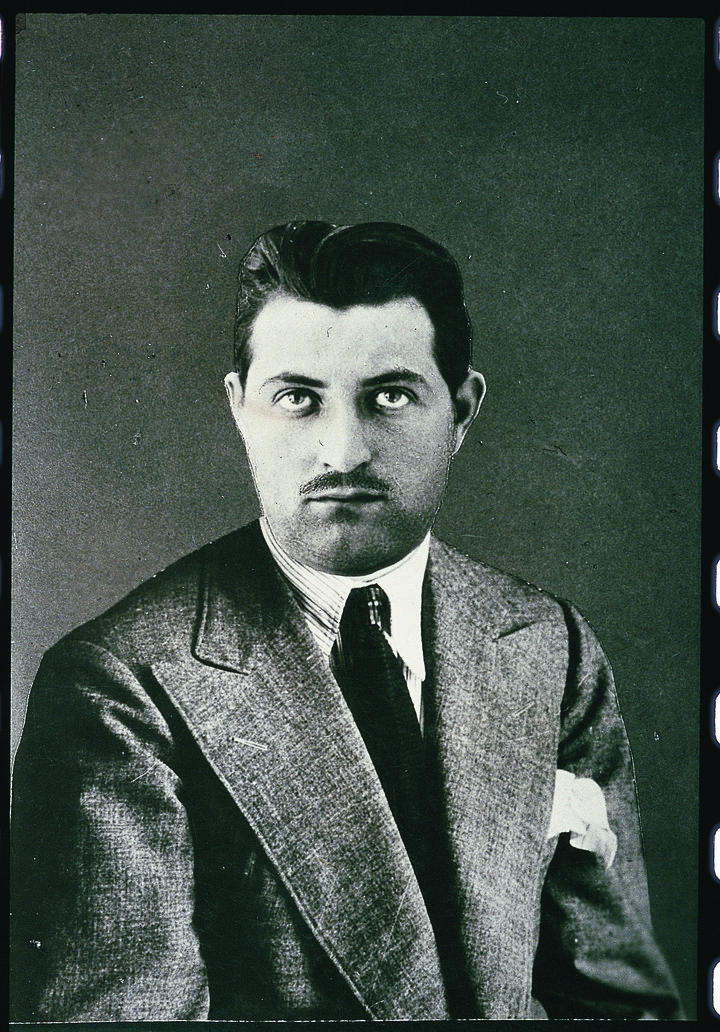
\includegraphics[width=0.5\textwidth]{../Images/SeverinoDiGiovanni.jpg}
 \caption{Severino Di Giovanni, el autor de este apunte. Un anarquista
   libertario, murió luchando por la libertad. Como él, otros miles han muerto
   para que nosotros gocemos de los derechos que tenemos. No te dejes engañar
   por los tristes pregoneros del egoísmo. Amá a tu prójimo y no olvides que si
   sus derechos se vulneran, los tuyos también. Ayudá a tu compañero de estudio,
 defendé tu universidad. }
 \end{figure}

\pagebreak
\tableofcontents
\newpage


\section{P1} 

\begin{myframe}
\textbf{(1)} Un geólogo recoge 10 especímenes de A y 12 de B. 15 son elegidos
al azar. De la función de probabilidad de masa del número de especímenes de tipo
A elegidos.
\end{myframe}
~


\textbf{Solución.} Sea $\Omega$ el espacio muestral, con cada $\omega \in \Omega$ una de las
posibles selecciones de $15$ de entre los $22$ especímenes. Claramente,

\begin{equation*}
  \left| \Omega \right| = \binom{22}{15}
\end{equation*}

Sea $X$ la variable aleatoria para el número de especímenes de tipo $A$ en una
selección aleatoria de $\Omega$. Claramente, para tener $X = k$, con $3 \leq k
\leq 10$, la selección debe ser tal que $k$ muestras sean de tipo $A$ y $15 - k$
muestras sean de tipo $B$. Luego 

\begin{equation*}
  P(X = k) = \frac{\binom{10}{k} \binom{12}{15 - k}}{\binom{22}{15}}
\end{equation*}




\pagebreak 

\begin{myframe}
\textbf{(2)} Sean $X, Y$ independientes y exponenciales con parámetros $\lambda,
\mu$ respectivamente. Computar $f_{X | Y}(x \mid y)$ y $P(X < Y)$.
\end{myframe}

~


  $(a)$ Recordemos que $f_{X \mid Y}(x \mid y) = \frac{f_{X, Y}(x,
  y)}{f_Y(y)}$. Como $X, Y$ son independientes, su densidad conjunta es el
  producto de las densidades, y tenemos $f_{X \mid Y}(x \mid y) = (f_X(x)
  f_Y(y))/f_Y(y) = f_X(x)$.

  $(b)$ Veamos que

  \begin{align*}
    P(X < Y) 
    &= \int_{\mathbb{R}} f_Y(y) \int_{-\infty}^y f_X(x) ~ dx ~ dy \\ 
    &=\int_\mathbb{R} \mathcal{I}_{(0, \infty)} \cdot \mu e^{-\mu y}
    \int_{-\infty}^y \mathcal{I}_{(0, \infty)} \lambda e^{-\lambda x} ~ dx ~ dy
    \\ 
    &=\int_0^\infty \mu e^{-\mu y}\int_0^y \lambda e^{-\lambda ~ x}
  \end{align*}

Ahora bien, con $w := -\lambda x, dw = -\lambda dx$, tenemos

\begin{align*}
  \int_0^y \lambda e^{-\lambda x} ~ dx 
  &= -\int_0^{w(y)}  e^w ~ dw \\ 
  &=-\int_0^{-\lambda y} e^w ~ dw \\ 
  &= - \left[ e^{-\lambda y} - e^0 \right] \\ 
  &=1 - e^{- \lambda y}
\end{align*}

Por lo tanto

\begin{align*}
P(X < Y) 
  &= \int_0^\infty \mu e^{-\mu y} \left( 1 - e^{-\lambda ~ y} \right) ~ dy \\ 
  &= \int_0^\infty \mu e^{-\mu y} ~ dy - \int_0^\infty \mu e^{-(\mu + \lambda) y
  } ~ dy \\ 
  &= \int_0^\infty f_{Y}(y) ~ dy - \frac{\mu}{\mu + \lambda}\int_0^\infty (\mu +
  \lambda)e^{-(\mu + \lambda) y} ~ dy \\ 
  &= 1 - \frac{\mu}{\mu + \lambda} \int_0^\infty f_{Z}(y) ~ dy &\left\{ Z \sim
  \mathcal{E}(\mu + \lambda) \right\}  \\ 
  &= 1 - \frac{\mu}{\mu + \lambda} \\ 
  &= \frac{\mu + \lambda}{\mu + \lambda} - \frac{\mu}{\mu + \lambda} \\ 
  &= \frac{\lambda}{\mu + \lambda}
\end{align*}

\pagebreak

\begin{myframe}
\textbf{(3)} Sean $X, Y$ independientes y exponenciales con el mismo parámetro
$\lambda$. Computar la densidad
condicional de $X$ dado que $X + Y = t$.
\end{myframe}

~

\textbf{Solución.} Por def. de densidad condicional, tomando $T := X + Y$,

  \begin{equation*}
    f_{X \mid T}(x\mid t) = \frac{f_{X, T}(x, t)}{f_T(t)} 
  \end{equation*}

Calculemos estas distribuciones.

\begin{align*}
  f_{X, T}(x, t) 
  &= P(X = x \cap X + Y = t) \\ 
  &= P(X = x \cap Y = t - x) \\ 
  &=P(X = x) \cdot P(Y = t - x) &\left\{ X, Y \text{ son independientes}
  \right\} \\ 
  &= f_X(x) \cdot f_Y(t - x) \\ 
  &= \lambda e^{-\lambda x} \mathcal{I}_{(0, \infty)}(x) \cdot \lambda e^{-\lambda(t - x)} ~ \mathcal{I}_{(0,
  \infty)}(t-x)\\ 
  &= \lambda^2e^{-\lambda t} ~ \mathcal{I}_{(0, \infty)}(t-x) \mathcal{I}_{(0,
  \infty)}(x) \\ 
  &= \lambda^2e^{-\lambda t} ~ \mathcal{I}_{(x, \infty)}(t) \mathcal{I}_{(0,
  \infty)}(x) \\ 
\end{align*}

El último paso se justifica porque $\mathcal{I}_{(0, \infty)}(t-x)\mathcal{I}_{(0,
\infty)}(x) = \mathcal{I}_{(0, \infty)}(x) \mathcal{I}_{(x, \infty)}(t)$. En
efecto, $t - x$ pertenece a $(0, \infty)$ si y solo si $t > x$. Ahora bien,

\begin{align*}
  f_T(t) 
  &= f_{X+Y}(t) \\ 
  &= \int_{\infty}^t f_X(x) f_Y(t - x) ~ dx &\left\{ X, Y \text{ independientes}
  \right\} \\ 
  &= \int_{-\infty}^t \mathcal{I}_{(0, \infty)} \cdot \lambda e^{-\lambda x}
  \cdot \mathcal{I}_{(0, \infty)}(t-x) \lambda
  e^{-\lambda(t - x)} ~ dx \\ 
  &=\int_0^t \lambda^2 e^{-\lambda t} \cdot 
  \mathcal{I}_{(x, \infty)}(t) ~ dx \\ 
  &=\lambda^2 e^{-\lambda  t} \int_0^t \mathcal{I}_{(x, \infty)}(t)~ dx \\ 
  &=\lambda^2 e^{-\lambda  t} \int_0^t 1 ~ dx \qquad (\star)\\ 
  &=t\lambda^2 e^{-\lambda  t} 
\end{align*}

El paso a $(\star)$ se justifica como sigue. Si la región de integración es $(0, t)$ y la variable de
integración es $x$, siempre se cumple que $x < t$, y por lo tanto
$\mathcal{I}_{(x, \infty)}(t) = 1$.

  \begin{equation*}
    \therefore \quad f_{X \mid T}(x\mid t) = \frac{f_{X, T}(x, t)}{f_T(t)} 
    = \frac{\lambda^2 e^{-\lambda t}\mathcal{I}_{(0, \infty)(x)}\mathcal{I}_{(x,
    \infty)}(t)}{t \lambda^2 e^{-\lambda t}} = \begin{cases}
      \frac{1}{t} & 0 \leq x \leq t  \\ 
      0 & c.c.
    \end{cases}
  \end{equation*}


\pagebreak 

\begin{myframe}
\textbf{(4)} Sean $N_1(t), N_2(t)$ procesos con $t \geq 0$ y tasas $\lambda = 1,
\mu = 2$ respectivamente. Sea $N(t) = N_1(t) + N_2(t)$. 

$(a)$ Calcular la probabilidad de que $N(1) = 2, N(2) = 5$.

$(b)$ Calcular la probabilidad de que $N_1(1) = 1$ dado $N(1) = 2$.

$(c)$ Calcular la probabilidad de que el segundo arribo en $N_1$ ocurra antes
que el tercer arribo en $N_2(t)$.
\end{myframe}

~

$(a)$ Es muy fácil porque $N(t)$ es un proceso de Poisson con parámetro $\lambda
+ \mu = 3$, con lo cual $P(N(t) = k) = e^{-3} \frac{3^k}{k!}$ para cualquier $k
\geq 0$ entero.

~ 

$(b)$ Claramente, si $N(1) = 2$, la probabilidad de que $N_1(1) = 1$ es la
probabilidad de que $N_2(1) = 1$.

\begin{align*}
  P(N_1(1) = 1 \mid N(1) = 2) 
  &= \frac{P(N_1(1) = 1 \cap N(1) = 2)}{P( N(1) = 2 )} \\ 
  &= \frac{ P(N_1(1) = 1 \cap  N_1(1) + N_2(1) = 2) }{P(N(1) = 2)} \\ 
  &= \frac{ P(N_1(1) = 1 \cap N_2(1) = 1) }{P(N(1) = 2)} \\ 
  &=\frac{ P(N_1(1) = 1) \cdot P(N_2(1) = 1) }{P(N(1) = 2)} &\left\{
  \text{Independencia de } N_1, N_2 \right\} 
\end{align*}

Ahora solo resta ver que 

\begin{equation*}
  e^{-\lambda ~ l} \frac{( \lambda l)^k}{k!} \leq e^{- \mu ~ l} \frac{( \mu l )^k}{k!} \iff
  e^{-\lambda l} \lambda^k \leq e^{-\lambda \mu} \mu^k \iff \lambda  \ln
  \lambda \geq \mu  \ln \mu
\end{equation*}

\begin{align*}
  P(N_1(1) = 1) &= e^{-1} \frac{1^1}{1!} = e^{-1} \approx 0.368 \\ 
  P(N_2(1) = 1)&= e^{-2} \frac{2^1}{1!} = 2e^{-2} \approx 0.27\\ 
  P(N(1) = 2) &= e^{-3} \frac{3^2}{2!} = \frac{9}{2}e^{-3} \approx 0.224
\end{align*}

\begin{equation*}
  \therefore P(N_1(1) = 1 \mid N(1) = 2) \approx \frac{0.368 \cdot 0.27}{0.224}
  = 0.443
\end{equation*}

Otra forma de calcularlo es usando el teorema de Bayes:

\begin{align*}
  P(N_1(1) = 1 \mid N(1) = 2) 
  &= \frac{P(N(1) = 1 \mid N_1(1) = 1) P(N_1(1) =
  1)}{P(N(1) = 1)} \\ 
  &= \frac{P(N_1(1) + N_2(1) = 1 \mid N_1(1) = 1) P(N_1(1) = 1)}{P(N(1) = 1)} \\ 
  &=\frac{ P(N_2(1) = 1) \cdot P(N_1(1) = 1) }{P(N(1) = 2)}
\end{align*}

que es lo mismo que tuvimos antes.

~

$(c)$ Se nos pide la probabilidad de que el segundo arribo en $N_1(t)$ ocurra antes
que el tercer arribo en $N_2(t)$. A primera vista no parece, pero este es
simplemente un problema de conteo. 

Primero, observemos que el evento "el segundo arribo en $N_1(t)$ ocurre antes
que el tercero de $N_2(t)$" es equivalente al evento "de $4$ eventos en $N(t)$,
al menos dos provienen de $N_1(t)$". Sea $\omega$ este evento.

La probabilidad de que un evento dado de $N(t)$ provenga de $N_1(t)$ es
$\frac{\lambda}{\lambda + \mu}$. La probabilidad de que un evento dado de $N(t)$
provenga de $N_2(t)$ es $\frac{\mu}{\lambda + \mu}$.

\begin{align*}
  \therefore ~ P(\omega) 
  &= \binom{4}{2} \frac{\lambda^2\mu^2}{( \lambda + \mu
  )^4} + \binom{4}{3} \frac{\lambda^3 \mu}{(\lambda + \mu)^4} +
  \binom{4}{4}\frac{\lambda^4}{(\lambda+ \mu)^4}
\end{align*}

Sustituyendo $\lambda, \mu$ por sus valores y calculando los binomiales, que son
fáciles, sale el resultado.

\pagebreak 

\begin{myframe}
\textbf{(5)} Sean $X, Y$ independientes con distribuciones de Poisson
parametrizadas bajo $\lambda, \mu$ respectivamente. Probar que 
$Z = X + Y \sim \mathcal{P}(\lambda + \mu)$.
\end{myframe}


Como son independientes, la distribución de su suma es dada por la "convolución"
discreta de sus distribuciones. Si con $\mathbb{N}$ denotamos los naturales y
el cero, entonces

\begin{align*}
  f_{Z}(z)  
  &=\sum_{k \in \mathbb{N} } p_X(k) p_Y(z - k)  \\ 
  &=\sum_{k \in \mathbb{N}} \left( e^{-\lambda} \frac{\lambda^k}{k!} \right)
  \left( e^{- \mu} \frac{\mu^{z - k}}{(z-k)!} \right)  \\ 
  &=e^{-\lambda }e^{-\mu} \sum_{k \in \mathbb{N}} \frac{\lambda^k
  \mu^{z-k}}{k!(z-k)!} \\ 
  &= \frac{\eta}{z!} \sum_{k \in \mathbb{N}} \lambda^k \mu^{z-k}\frac{z!}{k!(z -
k)!} &\left\{ \eta := e^{-\lambda }e^{-\mu} \right\}  \\ 
     &= \frac{\eta}{z!} \sum_{k\in \mathbb{N}} \lambda^k \mu^{z-k} \binom{z}{k}
\end{align*}

Ahora bien, como $Y \sim \mathcal{P}(\mu)$, $Im(Y) = \mathbb{N}$, y por lo tanto
$p_Y(u) = 0$ si $u < 0$. En otras palabras, dado un $k$ arbitrario, 
$p_Y(z - k) \neq 0 \iff z - k \geq 0 \iff k \leq z$.

\begin{equation*}
  &\therefore \frac{\eta}{z!} \sum_{k\in \mathbb{N}} \lambda^k \mu^{z-k}
  \binom{z}{k} 
  = \frac{\eta}{z} \sum_{k = 0}^z \lambda^k \mu^{z-k}\binom{z}{k} =
  \frac{\eta}{z!} (\lambda + \mu)^z = e^{-(\lambda + \mu)}\frac{(\lambda+\mu)^z}{z!}
\end{equation*}

por el teorema del binomio de Newton. 

$\therefore $ $Z \sim \mathcal{P}(\lambda + \mu)$. $\qquad \blacksquare$

\pagebreak 

\section{P3}

\begin{myframe}
\textbf{(2)} (Todas las variables en este problema son uniformes continuas e
independientes en
$(0, 1)$).
En un juego, se simula la variable aleatoria $U$.
Si $U < \frac{1}{2}$ se suman dos números aleatorios. Si $U \geq
\frac{1}{2}$, se suman tres. El resultado $X$ de cualquiera de estas sumas
es el puntaje, y se tiene éxito si $X \geq 1$.

~

$(a)$ Dar la probabilidad de ganar y $(b)$ escribir una simulación para estimar
la probabilidad de ganar.
\end{myframe}

~

$(a)$ Por ley de probabilidad total,

\begin{align*}
  &P(X_1 + X_2 \geq 1 \mid U < \frac{1}{2})P(U < \frac{1}{2}) + P(X_1 +
  X_2 + X_3 \geq 1\mid
  U \geq \frac{1}{2})P(U \geq \frac{1}{2}) \\ 
  =&P(X_1 + X_2 \geq 1)P(U < \frac{1}{2}) + P(X_1 + X_2 + X_3 \geq 1)P(U \geq
  \frac{1}{2})\\
  =&P(X_1 + X_2 \geq 1)\cdot \frac{1}{2} + P(X_1 + X_2 + X_3 \geq
  1)\cdot \frac{1}{2}
\end{align*}

Estudiemos $P(X_1 + X_2 = z)$. Veamos que si $z \in [0, 1]$, entonces

\begin{equation*}
  P(X_1 + X_2 = z) = \int_0^z f_{X_1}(x)f_{X_2}(z-x) ~ dx = \int_0^z 1 ~ dx 
  =z
\end{equation*}

Si $z \in (1, 2]$, entonces hacemos variar $X_1$ entre $[z-1, 1]$ y requerimos
$X_2 = z - X_1$:

\begin{equation*}
  P(X_1 + X_2 = z) 
  = \int_{z-1}^{1} f_{X_1}(x) f_{X_2}(z - x) ~  dx = 2 -z
\end{equation*}



\begin{equation*}
  \therefore ~ f_{X_1 + X_2}(x) = \begin{cases}
    x & 0 \leq x \leq 1 \\ 
    2 - x & 1 < x \leq 2 \\ 
    0 & c.c.
  \end{cases}
\end{equation*}

Por lo tanto,

\begin{equation*}
  P(X_1 + X_2 \geq 1) = \int_1^2 f_{X_1 + X_2}(x) ~ dx = \int_1^2(2-x) ~ dx =
  1 / 2
\end{equation*}

Resta ver que 

\begin{align*}
  P(X_1 + X_2 + X_3 \geq 1) 
  &= P(X_1 + X_2 \geq 1 - X_3) \\ 
  &=\int_0^1  P(X_1 + X_2 \geq 1 - z) P(X_3 = z) ~ dz &\left\{ \text{Por prob.
  total} \right\} \\ 
  &=\int_0^1 \left(1 - \frac{(1-z)^2}{2}\right) \cdot 1 ~ dz &\left\{ \text{Por }
  \star\right\} \\ 
  &=5 / 6
\end{align*}

dado que para $z \in [0, 1]$

\begin{equation*}
  ( \star ) \qquad P(X_1 + X_2 \geq 1 - z) = 1 - P(X_1 + X_1 \leq 1 - z) = 1 - \int_0^{1-z} x ~ dx = 1 - \frac{ (1-z)^2 }{2}
\end{equation*}

\begin{align*}
  \therefore  ~ ~ ~
  &P(X_1 + X_2 \geq 1)\cdot \frac{1}{2} + P(X_1 + X_2 + X_3 \geq
  1)\cdot \frac{1}{2} \\
  = &\frac{1}{2} \cdot \frac{1}{2} + \frac{5}{6} \cdot
  \frac{1}{2}  \\
  = &\frac{1}{4} + \frac{5}{12} \\
  =&\frac{2}{3}
\end{align*}

~

$(b)$ En Python, 


\begin{verbatim}[python]
from random import uniform

def sim_2(n):

  wins = 0

  # S = summation of uniform rvs
  def S(k):
    return sum( [uniform(0, 1) for _ in range(k)] )

  for _ in range(n):

    u = uniform(0, 1)
 
    X = S(2) if u < 0.5 else S(3)
    wins = wins + 1 if X >= 1 else wins

  return wins/n
\end{verbatim}


\pagebreak 

\begin{myframe}
\textbf{(3)} Las máquinas tragamonedas usualmente generan un premio cuando hay un acierto. Supongamos que se genera el acierto con el siguiente esquema: se genera un número aleatorio, y

\begin{itemize}
\item si es menor a un tercio, se suman dos nuevos números aleatorios
\item si es mayor o igual a un tercio, se suman tres números aleatorios .
\end{itemize}

Si el resultado de la suma es menor o igual a 2, se genera un acierto.

~

$a)$ ¿Cuál es la probabilidad de acertar? $(b)$ Simular.
\end{myframe}


Sea $Z_n = \sum_{i=1}^n U_i$ con $U_i \sim \mathcal{U}(0, 1)$ para $1 \leq i
\leq n$. Por ley de probabilidad total, se llega con facilidad a

\begin{equation*}
  P(\text{Ganar}) = P(Z_2 \leq 2) \cdot \frac{1}{3} + P(Z_3 \leq 2) \cdot
  \frac{2}{3}
\end{equation*}

Claramente, $P(Z_2 \leq 2) = 1$, con lo cual solo queda computar $P(Z_3 \leq
2) = P(Z_2 \leq 2 - U_3)$. La densidad de $Z_2$ fue calculada en el punto
$\textbf{(2)}$. Para calcular $P(Z_3 \leq 2)$, podemos hacer variar a $U_3$ en
todo el rango $[0, 1]$ y a $Z_2$ en todo el rango $[ 0, 2 - U_3 ]$:

\begin{align*}
  P(Z_3 \leq Z_2) 
  &= P(Z_2 \leq 2 - U_3) \\ 
  &=\int_0^1 P(U_3 = z) \int_{0}^{2-z} f_{Z_2}(x) ~ dx ~ dz \\ 
  &=\int_0^1 \left[ \int_0^1 f_{Z_2}(x) ~ dx + \int_1^{2 - z} f_{Z_2}(x) ~ dx
  \right] ~ dz \\ 
  &=\int_0^1 \left[ \int_0^1 x ~ dx + \int_1^{2-x}(2-x) ~ dx  \right] ~ dz \\ 
  &= \int_0^1 \left[ \frac{1}{2} - \frac{z^2}{2} + \frac{1}{2}\right]  ~ dz \\ 
  &=\int_0^1 1 - \frac{z^2}{2} ~ dz \\ 
  &= 5 / 6
\end{align*}


Una forma alternativa de calcular esta probabilidad es hacer variar a $Z_2$ en
todo el rango $[0, 2]$ y luego hacer variar a $U_3$ en todo el rango $[0, 2 -
Z_2]$:

\begin{align*}
  P(Z_3 \leq 2) 
  &=P(Z_2 \leq 2 - U_3)\\
  &= \int_0^2 f_{Z_2}(x) \int_0^{2-x} f_{U_3}(y) ~ dy ~ dx \\ 
  &= \int_0^1 f_{Z_2}(x) \int_0^{1} f_{U_3}(y) ~ dy ~ dx + \int_1^2 f_{Z_2}(x)
  \int_0^{2-x} f_{U_3}(y) ~ dy ~ dx &\left\{ \text{Por } \star \right\}  \\
                                    &=\int_0^1 x \int_0^1 1 ~ dy ~ dx +
                                    \int_{1}^2 (2-x) \int_0^{2 - x} 1 ~ dy ~ dx\\
  &=\int_0^1 x ~ dx + \int_1^2 (2-x)^2 ~ dx \\
  &=\frac{1}{2} + \frac{1}{3} \\ 
  &= \frac{5}{6}
\end{align*}

\begin{myframe}
  ($\star$) Si $Z_2$ varía en $[0, 1]$, $Z \leq 2 - U_3$ para cualquier valor de
  $U_3$, con lo cual hacemos a $U_3$ variar en todo el rango $[0, 1]$.  Pero si
  $Z_2$ varía en $[1, 2]$, entonces $U_3$ solo puede tomar valores en $[0, 2 -
  Z_2]$.
\end{myframe}

\begin{align*}
  \therefore \qquad P(\text{Ganar}) 
  &= P(Z_2 \leq 2) \cdot \frac{1}{3} + P(Z_3 \leq 2) \cdot
  \frac{2}{3} \\ 
  &= \frac{1}{3} + \frac{5}{6}\frac{2}{3} \\ 
  &= 0.\overline{8}
\end{align*}

~

$(b)$En Python, una implementación posible es:

\begin{verbatim}
from random import uniform

def sim_3(n):
  wins = 0 

  # S = summation of uniform r.vs
  def S(k): 
    return sum( [uniform(0, 1) for _ in range(k)] )

  for _ in range(n):
    u = uniform(0, 1)
    X = S(2) if u < 1/3 else S(3)
    wins = wins + 1 if X <= 2 else wins

  return wins/n
\end{verbatim}


\pagebreak 

\begin{myframe}
(\textbf{4}) Un supermercado posee 3 cajas. Por una cuestión de ubicación, el
40\% de los clientes eligen la caja 1 para pagar, el 32\% la caja 2, y el 28\%
la caja 3. 

El tiempo que espera una persona para ser atendida en cada caja
distribuye exponencial con medias de 3, 4 y 5 minutos respectivamente. 

~

$(a)$ ¿Cuál es la probabilidad de que un cliente espere menos de 4 minutos para ser
atendido? 

$(b)$ Si el cliente tuvo que esperar más de 4 minutos. ¿Cuál es la
probabilidad de que el cliente haya elegido cada una de las cajas? 


$(c)$ Simule el
problema y estime las probabilidades anteriores con 1000 iteraciones.
\end{myframe}

~ 

Recordemos que la media de la exponencial es $1 / \lambda$, es decir que
$\lambda_1 = 1 / 3, \lambda_2 = 1 / 4, \lambda_3 = 1 / 5$.

El evento "un cliente espera menos de $4$ minutos en ser atendido" se divide en
un sub-eventos correspondiente por cada caja. Más formalmente, si $T$ es el
tiempo de espera de un cliente arbitrario, y $C_i$ el evento de que el cliente
elige la i-ésima caja, entonces por ley de probabilidad total:

\begin{equation*}
  P(T \leq 4) = \sum_{i=1}^3 P(C_i)P(T \leq 4 \mid C_i) = \sum_{i=1}^3 P(C_i)
  P(X_i \leq 4)
\end{equation*}

donde $X_i$ es una exponencial con parámetro $\lambda_i$. En general, 

\begin{equation*}
  \int_0^4 \lambda_i e^{-\lambda_i x} ~dx = 1 - e^{-4\lambda_i}
\end{equation*}

de lo cual se sigue: 

\begin{equation*}
  P(X_i \leq 4) = \begin{cases}
    0.736 & i = 1 \\ 
    0.632 & i = 2\\ 
    0.55 & i = 3
  \end{cases}
\end{equation*}

\begin{equation*}
  \therefore P(T\leq 4) = 0.40 \cdot 0.736 + 0.32 \cdot 0.632 + 0.28 \cdot 0.55
  = 0.65064
\end{equation*}

~

$(b)$  Sale fácil con teorema de Bayes y los resultados de $(a)$:

  \begin{equation*}
    P(C_i \mid T \leq 4) 
    &= \frac{P(T \leq 4 \mid C_i)P(C_i)}{P(T \leq 4)}
  \end{equation*}

~

$(c)$ En Python,

\begin{verbatim}
from numpy.random import exponential
from random import uniform

def sim_4(n):

  wins = 0
  rates = [1/3, 1/4, 1/5]

  def choose_rate(x):
    if x <= 0.4:
      return 0 
    return 1 if u <= 0.4 + 0.32 else 2

  for _ in range(n): 

    u = uniform(0, 1)
    rate = rates[choose_rate(u)]

    e = exponential(1/rate)

    wins = wins + 1 if e <= 4 else wins

  return wins/n 


\end{verbatim}

\pagebreak 

\begin{myframe}
\textbf{(5)} Calcule con el método de Monte Carlo y escriba simulaciones para
cada una de las siguientes integrales. 
\end{myframe}

~ 

\begin{myframe}
$(a)$ $\int_0^1 (1-x^2)^{3 / 2} ~ dx$
\end{myframe}

Sea $f_U(x)$ la densidad de $U \sim \mathcal{U}(0, 1)$. Entonces 

\begin{equation*}
  \theta := \int_0^1(1-x^2)^{3 / 2} ~ dx = \int_0^1 (1-x^2)^{3 / 2} f_U(x) ~ dx =
  \mathbb{E}\left[ g(U) \right] 
\end{equation*}

con $g(x) = (1-x^2)^{3 / 2}$. Por lo tanto, $\theta \approx \frac{1}{n}
\sum_{i=1}^n g(u_i)$ con $u_1, \ldots, u_n$ realizaciones de $U_1, \ldots, U_n
\sim \mathcal{U}(0, 1)$. Es decir, 

\begin{equation*}
  \theta \approx \frac{1}{n} \sum^n (1 - u_i^2)^{3 / 2}
\end{equation*}

En Python,

\begin{verbatim}
from random import uniform
def sim_5a(n):
  uniforms = [uniform(0, 1) for _ in range(n)]
  return 1/n * sum( [ (1 - u**2)**1.5  for u in uniforms ] )

\end{verbatim}

\pagebreak


\begin{myframe}
$(b) \int_2^3 \frac{x}{x^2-1} ~ dx$
\end{myframe}


Si hacemos $u = x - 2$, tal que $du = dx$ y $x = 2 + u$, tenemos 

\begin{equation*}
  \theta := \int_2^3 \frac{x}{x^2 - 1} ~ dx = \int_0^1 \frac{2+u}{(2+u)^2 - 1} ~ du =
  \int_0^1 \frac{2+u}{u^2 - 4u + 3}
\end{equation*}

Entonces $\theta = \int_0^1 g(x)f_U(x) ~ dx = \mathbb{E}\left[ g(U) \right] $
con $U \sim \mathcal{U}(0, 1), g(x) = \frac{2+x}{(2+x)^2 - 1}$. 

\begin{equation*}
  \therefore ~ \theta \approx \frac{1}{n}\sum_{i=1}^n \frac{2 + u_i}{u_i^2
  -4u_i + 3}
\end{equation*}

donde $u_1, \ldots, u_n$ son realizaciones de $U_1, \ldots, U_n \sim
\mathcal{U}(0, 1)$ independientes para $n \geq 1$. En Python, 

  
\begin{verbatim}
def sim_5b(n):
  uniforms = [uniform(0, 1) for _ in range(n)]
  return 1/n * sum( [ (2 + u)/((2+u)**2 - 1) for u in uniforms ] )
\end{verbatim}

Con $n = 1000$ obtuve $\theta \approx 0.487$, y el valor real de la integral es $\theta = 0.49$.

\pagebreak

\begin{myframe}
$(c) \int_0^\infty x(1+x^2)^{-2} ~ dx$
\end{myframe}


Sea $u := \frac{1}{x + 1}$, de manera que 

\begin{equation*}
  du = -\frac{1}{(x+1)^2} ~ dx = -u^2 ~ dx, \qquad x = \frac{1-u}{u} =
  \frac{1}{u} - 1
\end{equation*}

Entonces 

\begin{align*}
  \theta := \int_0^\infty g(x) ~ dx = -\int_0^1 \frac{g(\frac{1}{u} - 1)}{u^2}
  ~ du = -\int_0^1 \frac{(\frac{1}{u} - 1)(1 + (\frac{1}{u} - 1)^2)^{-2}}{u^2} ~
  du
\end{align*}

Luego 

\begin{equation*}
  \theta = -\int_0^1 \psi(u) f_U(u) ~ du = -\mathbb{E}\left[ \psi(U) \right] 
\end{equation*}

con $\psi(u) = g(\frac{1}{u} - 1) / u^2$ y $U \sim \mathcal{U}(0, 1)$. En
consecuencia, 

\begin{equation*}
  \theta \approx \frac{1}{n}\sum_{i=1}^n \psi(u_i)
\end{equation*}

donde $u_1, \ldots, u_n$ son realizaciones de $U_1, \ldots, U_n \sim
\mathcal{U}(0, 1)$ independientes (no confundir con $u$, la variable de
integración) y $n \geq 1$. En Python, 

\begin{verbatim}
def sim_5c(n):
  uniforms = [uniform(0, 1) for _ in range(n)]

  def h(u):
    return (1/u - 1)*(1 + (1/u - 1)**2)**(-2) * (1/u**2)

  return 1/n * sum( [h(u) for u in uniforms] )
\end{verbatim}

Con $n = 1000$, la simulación dio $\varphi \approx 0.504$, y el valor real de la
integral es $\theta = \frac{1}{2}$.

\pagebreak

\begin{myframe}
$(d) \int_{-\infty}^\infty e^{-x^2} ~ dx$
\end{myframe}


Let $g(x) := e^{-x^2}$. Clearly, $g(-x) = e^{-(-x^2)} = g(x)$, which means $g$
is symmetric.

$\therefore ~ \int_{-\infty}^\infty e^{-x^2} ~ dx = 2\int_0^\infty e^{-x^2} ~
dx$. If we let 

\begin{equation*}
  \psi = \frac{1}{x+1}, \qquad d \psi = -\psi^2, \qquad x = \frac{1}{\psi}-1
\end{equation*}

Entonces

\begin{equation*}
  \theta := 2\int_0^\infty e^{-x^2} = 2\int_0^1 \frac{\exp\left(-\left(\left(\frac{1}{\psi} -
  1\right)^2\right)\right)}{\psi^2} f_U(\psi) ~ d\psi
\end{equation*}

donde $f_U$ es la densidad de $U \sim \mathcal{U}(0, 1)$. $\therefore
\theta = \mathbb{E}\left[ h(U) \right] $ con $h(x) =
\exp\left(-\left(\left(\frac{1}{x}-1\right)^2\right) /
x^2$. 

\begin{equation*}
  \therefore \quad \theta \approx \frac{1}{n}\sum_{i=1}^n 
  \frac{\exp\left(-\left(\left(\frac{1}{u_i} - 1\right)^2\right)\right)}{u_i^2}, \qquad n \geq 1
\end{equation*}

con $u_1, \ldots, u_n$ realizaciones de $U_1, \ldots, U_n \sim \mathcal{U}(0,
1)$. En Python,

\begin{verbatim}
from math import exp 
from random import uniform
  
def sim_5d(n):
    def h(u):
        return exp(-(( 1/u - 1 )**2)) / (u**2)

    uniforms = [uniform(0, 1) for _ in range(n)]
    return 2*sum([ h(u) for u in uniforms ]) / n
\end{verbatim}

La simulación con $n = 1000$ dio $\theta \approx 1.73$ que es casi exactamente
$\sqrt{\pi}$, el verdadero valor.

\begin{myframe}
\textbf{Observación.} El ejercicio se puede resolver aplicando directamente la
sustitución sin notar que $g$ es simétrica, aunque se dan pasos previos algo más
engorrosos:

\begin{align*}
  \int_{-\infty}^\infty g(x) ~ dx 
  &= \lim_{t \to -\infty}\int_t^0 g(x) ~dx +
  \lim_{t \to \infty} \int_0^\infty g(x) ~ dx \\ 
  &=-\int_{\lim_{t \to -\infty} \psi(t)}^0 \frac{ g(\frac{1}{\psi} - 1) }{\psi^2}
  ~ d\psi - \int_0^{ \lim_{t \to \infty} \psi(t)} 
  \frac{g(\frac{1}{\psi} - 1)}{\psi^2} ~ d\psi \\ 
  &=\int_0^1 \frac{g(\frac{1}{\psi} - 1)}{\psi^2} ~ d\psi + \int_0^1
  \frac{g(\frac{1}{\psi} - 1)}{\psi^2} ~ d\psi \\ 
  &= 2 \int_0^1 \frac{g(\frac{1}{\psi} - 1)}{\psi^2} ~ d\psi
\end{align*}

A partir de acá todo es igual.
\end{myframe}


\pagebreak

\begin{myframe}
$(e)$ $\theta := \int_0^1 \int_0^1 \exp(( x+y )^2) ~ dx ~ dy$
\end{myframe}


Let $X, Y \sim \mathcal{U}(0, 1)$ independent with densities $f_Y, f_U$. Clearly, their
joint density function is 

\begin{equation*}
  f_{X, Y}(x, y) = f_X(x)f_Y(y) = \mathcal{I}_{(0, 1) \times (0, 1)}
\end{equation*}

Then 

\begin{equation*}
  \theta = \int_0^1 \int_0^1 g(x, y) f_{X, Y}(x, y) ~ dx ~ dy = \mathbb{E}\left[
  g(X, Y)\right] 
\end{equation*}

\begin{equation*}
  \therefore \quad \theta \approx \frac{1}{n} \sum_{i=1}^{n} g(x_i, y_i), \qquad
  n \geq 1
\end{equation*}

where $(x_1, y_1), \ldots, (x_n,y_n)$ are realizations of $(X_1, Y_1),
\ldots, (X_n, Y_n)$, with $X_i, Y_i \sim \mathcal{U}(0, 1)$ for $1 \leq i \leq
n$.

In Python,

\begin{verbatim}
from math import exp 
from random import uniform 

def sim_5e(n):
    def g(x, y):
        return exp((x+y)**2)
    
    X = [uniform(0, 1) for _ in range(n)]
    Y = [uniform(0, 1) for _ in range(n)]

    return sum([ g(x, y) for x, y in zip(X, Y) ]) / n
\end{verbatim}

With $n = 100000$, the estimation was $4.902$, and the true value of the
integral according to Wolfram Alpha is $4.899$.


\pagebreak 

\begin{myframe}
\textbf{(7)} Definamos 

\begin{equation*}
  N = \min_{n} \left\{ n : \sum_{i=1}^n U_i > 1 \right\}, \qquad U_i \sim
  \mathcal{U}(0, 1)
\end{equation*}

$(a)$ Estimar $\mathbb{E}[N]$ generating $n$ values for $N$.

$(b)$ Calculate $E[N]$.

\end{myframe}


Notemos que $Im(N) = \left\{ 2, 3, \ldots \right\} $. Calculemos $p_N(n)$ la
función de probabilidad de masa de $N$. Para ello, observemos que 

\begin{equation*}
  P(N = n) = P\left(\sum_{i=1}^{n-1} U_i \leq 1 \cap U_n > 1 - \sum_{i=1}^{n-1}
  U_i\right)
\end{equation*}

Sea $X(n) = \sum_{i=1}^n U_i$ y, para simplificar la notación, usemos
$\varphi(n, x) := P(X(n) \leq x)$ para $x \geq 0$. Es decir, $\varphi(n, x)$ es
la función de probabilidad acumulada de $X(n)$. Entonces, la expresión de arriba
nos queda

\begin{equation*}
  P(N = n) = P(X(n-1) < 1 \cap U_n > 1 -X(n-1)) 
\end{equation*}

De acuerdo con la ley de probabilidad total,


\begin{align*}
  \varphi(n, x) 
  &= P(X(n) \leq x) \\
  &= P(U_n \leq x - X(n-1)) \\
  &= \int_{\mathbb{R}} P(U_n \leq x-z) P\left( X(n-1) = z \right) ~ dz \\ 
  &=\int_0^{x} (x-z) \frac{d}{dz} \varphi(n-1, z) ~ dz
\end{align*}

donde estamos utilizando el hecho de que la función de densidad es la derivada
de la función de probabilidad acumulada. Esta expresión recursiva de $\varphi(n, x)$
nos permite avanzar: si restringimos $x \in [0, 1]$,


\begin{align*}
  \varphi(2, x) 
  &= \int_0^x(x-z)\frac{d}{dz}\varphi(1, z) ~ dz \\
  &=\int_0^x(x-z) ~ dz \\ 
  &= \frac{x^2}{2}
\end{align*}

Siguiendo probando casos, obtenemos

\begin{align*}
  f(x, 3) &= \int_0^x(x-z)z ~ dz = \frac{x^3}{6} \\
  f(x, 4) &= \int_0^x(x-z)\frac{z^2}{2} ~ dz = \frac{x^4}{24} \\
          &\vdots \\ 
  f(x, n) &= (x-t) \frac{d}{dz}\varphi(x, n-1)(x:=z) ~ dz = \frac{x^n}{n!}
\end{align*}

Es decir, obtenemos una expresión general para la probabilidad acumulada de
$X(n)$, de lo cual se deduce que la densidad de $X(n)$ es 

\begin{equation*}
  \psi(n, x) = \frac{d}{dx} \frac{x^n}{n!} = \frac{nx^{n-1}}{n!} =
  \frac{x^{n-1}}{(n-1)!} = \varphi(n-1, x), \qquad 0 \leq x \leq 1
\end{equation*}

Por lo tanto,

\begin{align*}
  P(N = n) 
  &= P(X(n-1) < 1 \cap U_n > 1 -X(n-1)) \\ 
  &=\int_0^1 \psi(n-1, x) P(U_n > 1 - x) ~ dx \\ 
  &=\int_0^1 \frac{x^{n-2}}{(n-2)!}(1 - P(U_n \leq 1-x)) ~ dx \\ 
  &=\frac{1}{(n-2)!}\int_0^1  x^{n-1} ~ dx \\ 
  &=\frac{1}{(n-2)!} \frac{1^n}{n} \\ 
  &= \frac{1}{n(n-2)!}
\end{align*}

Por lo tanto, 

\begin{equation*}
  \mathbb{E}\left[ N \right] = \sum_{i=2}^\infty \frac{1}{(n-2)!} =
  \sum_{i=0}^\infty \frac{1}{n!} = e
\end{equation*}

La simulación está de acuerdo, porque en Python 

\begin{verbatim}
def sim_7(iterations):

  counts = []
  n, s = 0, 0

  for _ in range(iterations):
    while s <= 1:
      n += 1
      s += uniform(0, 1)
    counts.append(n)
    n, s = 0, 0
 
  return sum(counts)/len(counts)
\end{verbatim}

nos devuelve siempre aproximadamente $e$.

\pagebreak 

\begin{myframe}
$\textbf{(8)}$ Sea  

\begin{equation*}
  N = \max_{n} \left( \prod_{i=1}^n U_i \geq e^{-3} \right) 
\end{equation*}

con $\prod_{i=1}^0 U_i = 1$. Estimar mediante simulaciones $E[N]$ y $P(N = n)$
para $0 \leq n \leq 6$.

\end{myframe}
~

Estimar con simulaciones es aburrido y fácil. Más vale pensemos en el problema y
tratemos de dar $p_N$, la función de probabilidad de masa de $N$, y con ella
$\mathbb{E}\left[ N \right] $ de manera analítica.

Claramente, 

\begin{align*}
  P(N = n) 
  &= P \left( \prod_{i=1}^{n-1} U_i \geq e^{-3} \cap U_n \cdot \prod_{i=1}^{n-1}
  U_i < e^{-3}\right) \\ 
  &= P \left( \prod_{i=1}^{n-1} U_i \geq e^{-3} \cap U_n  <
    \frac{e^{-3}}{\prod_{i=1}^{n-1}U_i }\right) 
\end{align*}

Para simplificar la notación, hagamos $X(n) := \prod_{i=1}^n U_i$ y $\varphi(n,
x) = P(X(n) \leq x)$ para $x \in [0, 1]$. Es decir, $\varphi$ es la CDF de
$X(n)$. Asumimos que $X(0) = 1$, con lo cual $\varphi(0, x) = 1$. Es fácil ver
que $\varphi(1, x) = x$. Veamos además que 

\begin{align*}
  \varphi(2, x) 
  &= P(U_1 U_2 \leq x) \\ 
  &= P(U_1 \leq \frac{x}{U_2}) \\ 
  &= \int_0^1 P(U_1 \leq \frac{x}{z}) P(U_2 = z) ~ dz  \\ 
  &= \int_0^1 P\left( U_1 \leq \frac{x}{z} \right)  ~ dz
\end{align*}

Como $x / z \leq 1$ para $z \in [x, 1]$ y $x / z > 1$ para $z \in [0, x)$,

\begin{align*}
  \int_0^1 P\left( U_1 \leq \frac{x}{z} \right) ~ dz 
  &=\int_0^x P\left( U_1 \leq \frac{x}{z} \right) ~ dz + \int_x^1 P\left( U_1
  \leq \frac{x}{z} \right) ~ dz \\ 
  &= \int_0^x 1 ~ dz + \int_x^1 \frac{x}{z} ~ dz \\ 
  &= x + x \Big[ \ln z\Big]_x^1 \\ 
  &= x - x \ln x
\end{align*}

\begin{myframe}
  Una forma alternativa de dar con la probabilidad buscada es la siguiente:
  
\begin{align*}
  \varphi(2, x) 
  &= P(U_1 U_2 \leq x)  \\ 
  &=\int_0^x \int_0^1 ~ dy ~ dz + \int_x^1 \int_{0}^{x / z} ~ dy ~ dz \\ 
  &=\int_0^x ~ dz + \int_{x}^1 \frac{x}{z} ~ dz \\ 
  &= x + x \int_x^1 \frac{1}{z} ~ dz \\ 
  &= x + x \Big[ \ln z \Big]_{x}^1 \\ 
  &= x + x(\ln 1 - \ln x) \\ 
  &= x - x \ln x
\end{align*}

Esta forma es más simple en este caso particular, pero la que usamos antes
es más útil para el caso general.
\end{myframe}

Generalizando, llegamos a

\begin{align*}
  \varphi(n, x) 
  &= P\left(\prod_{i=1}^{n-1} U_i \leq \frac{x}{U_n}\right)  \\ 
  &= \int_0^1 \varphi\left(n-1, \frac{x}{z}\right) P(U_n = z) ~ dz \\ 
  &=\int_0^1 \varphi\left(n-1, \frac{x}{z}\right) ~ dz \\ 
  &=\int_0^x \varphi \left( n - 1, \frac{x}{z} \right) ~ dz + \int_x^1 \varphi
  \left( n - 1, \frac{x}{z} \right) \\ 
  &= \int_0^x 1 ~ dz + \int_x^{1} \varphi\left( n-1, \frac{x}{z} \right)  \\ 
  &= x + \int_x^1 \varphi\left( n-1, \frac{x}{z} \right) 
\end{align*}

Entonces, usando el hecho de que conocemos $\varphi(2, x)$, tenemos 

\begin{align*}
  \varphi(3, x) 
  &= x + \int_x^1 \varphi(2, \frac{x}{z}) ~ dz  \\ 
  &=x + \int_x^1 \frac{x}{z}-\frac{x}{z} \ln \frac{x}{z} \\ 
  &= x - x\ln x + \frac{x}{2} \ln^2 x
\end{align*}

\begin{align*}
  \varphi(4, x) 
  &= x + \int_x^1 \varphi(3, \frac{x}{z}) ~ dz  \\ 
  &=
  x + \int_x^1 \frac{x}{z} -\frac{x}{z} \ln\left( \frac{x}{z} \right) + \frac{x}{2z} \ln^2 \left( \frac{x}{z} \right)   \\ 
  &=x - x \ln x + \frac{x \ln^2 x}{2} - \frac{x \ln^3 x}{6}
\end{align*}

Vistos estos resultados, notamos (aunque no demostramos formalmente) que:

\begin{equation*}
  \varphi(n, x) = \sum_{k=0}^{n-1} \left( -1 \right)^{k} \frac{x \ln^k x}{k!}
\end{equation*}

Por lo tanto, la función de probabilidad de masa $\psi(n, x)$ del producto de $n$ uniformes
aleatorias es $\frac{d}{dx}\varphi(n, x)$, que es


\begin{align*}
  &\sum_{k=0}^{n-1}(-1)^{k} 
  \frac{\ln^k x + k \ln^{k-1} x}{k!} \\
  =&1 - (\ln x + 1) + \left(\ln x + \frac{ \ln^2 x }{2}\right) -
  \left( \frac{\ln^3 x}{6} + \frac{1}{2}\ln^2 x \right)  + \ldots \\ 
  =& (-1)^{n-1} \frac{\ln^{n-1} x}{(n-1)!}  &\left\{ \text{Suma telescópica} \right\} \\ 
\end{align*}
Luego 


\begin{align*}
  P(N = n) 
  &= P \left( \prod_{i=1}^{n-1} U_i \geq e^{-3} \cap U_n \cdot \prod_{i=1}^{n-1}
  U_i < e^{-3}\right) \\ 
  &= P \left( \prod_{i=1}^{n-1} U_i \geq e^{-3} \cap U_n  < \frac{e^{-3}}{\prod_{i=1}^{n-1}U_i < e^{-3}}
    \right) \\ 
  &= \int_{e^{-3}}^1 P(U_n < \frac{e^{-3}}{z}) P\left( \prod_{i=1}^{n-1} U_i
  = z \right) ~ dz \\ 
  &=\int_{e^{-3}}^1 \left( \frac{e^{-3}}{z} \right) \psi(n-1, z) ~ dz \\ 
  &=\int_{e^{-3}}^1 \left( \frac{e^{-3}}{z} \right) (-1)^{n-2} 
  \frac{\ln^{n-2} z}{(n-2)!} ~ dz \\ 
  &= \frac{ (-1)^{n-2}e^{-3} }{(n-2)!}\int_{e^{-3}}^1
  \frac{ \ln^{n-2} z }{z} ~ dz \\ 
  &= \frac{ (-1)^{n-2}e^{-3} }{(n-2)!} \left( - \frac{(-3)^{n-1}}{n-1} \right)
  \\ 
  &= \frac{3^{n-1}e^{-3}}{(n-1)!} \\ 
  &= \frac{3^{n-1}}{e^3(n-1)!}
\end{align*}

Por lo tanto, 

\begin{align*}
  \mathbb{E}\left[ N \right] 
  &= \sum_{k=1}^\infty \frac{k 3^{k-1}}{e^{3}(k-1)!}\\
  &=\frac{1}{e^3} \sum_{k=0}^\infty 3^{k} \frac{k+1}{k!} \\
  &=\frac{1}{e^3}\left(\sum_{k=0}^\infty k \frac{3^k}{k!} + \sum_{k=0}^\infty
  \frac{3^k}{k!} \right) \\ 
  &=\frac{1}{e^3}\left(\frac{1}{e^{-3}}\sum_{k=0}^\infty k \cdot e^{-3} \frac{3^k}{k!} + \sum_{k=0}^\infty
  \frac{3^k}{k!} \right)
\end{align*}

Ahora somos pillos y vemos que la primera sumatoria es el valor
esperado de una Poisson con parámetro $\lambda = 3$, y por lo tanto es 
$3$. la otra sumatoria es $e^3$, dado que $e^x = \sum_{k=0}^\infty
\frac{x^k}{k!}$. Como $1 / e^{-3} = e^3$,

\begin{equation*}
  \therefore ~ \mathbb{E}\left[ N \right] = \frac{1}{e^3}(3e^3 + e^3) =
  \frac{1}{e^3} \cdot 4e^3 = 4
\end{equation*}

Este valor coincide con la estimación de la siguiente simulación:

\begin{verbatim}
def sim_9(iterations):

  counts = []
  n, s = 0, 1

  for _ in range(iterations):
    while s >= exp(-3):
      n += 1
      s *= uniform(0, 1)
    counts.append(n)
    n, s = 0, 1
 
  return sum(counts)/len(counts)
  
\end{verbatim}




\pagebreak 

\begin{myframe}
\textbf{(9)} Un juego consiste en dos pasos. En el primer paso se tira un dado
convencional. Si sale 1 o 6 tira un nuevo dado y se le otorga al jugador como
puntaje el doble del resultado obtenido en esta nueva tirada; pero si sale 2, 3,
4 o 5 en la primer tirada, el jugador debería tirar dos nuevos dados, y
recibiría como puntaje la suma de los dados. Si el puntaje del jugador excede
los 6 puntos entonces gana.

$(a)$ Calcular la probabilidad de que un jugador gane.  

$(b)$ Estimar mediante simulación.
\end{myframe}

~ 


Sea $X = 1$ si el primer dado es 1 o 6, $X = 0$ si el primer dado es 2, 3, 4 o
5. Claramente $X$ es una Bernoulli con $p = 1 / 3$. Entonces, de acuerdo con la
ley de probabilidad total,

\begin{align*}
  P(\text{Ganar}) = P(2U > 6 \mid X = 1 )P(X = 0) + P(U_1 + U_2 > 6 \mid X = 0
  )P(X = 0 )
\end{align*}

con $U, U_2, U_3$ uniformes discretas en $\left\{ 1,\ldots,6 \right\} $.
Claramente, $U_1 + U_2 > 6$ y $2U$ son independientes de $X$. Por lo tanto 

\begin{equation*}
  P(\text{Ganar}) = P(U > 3) 1 / 3 + P(U_1 + U_2 > 6) 2 / 3
\end{equation*}

Ahora bien, $P(U_1 + U_2 > 6) = 1 - P(U_1 \leq 6 - U_2)$, y

\begin{align*}
  P(U_1 \leq 6 - U_2) 
  &= \sum_{k=1}^6 P(U_1 \leq 6 - k)P(U_2 = k) \\ 
  &=\sum_{k=1}^6 \frac{6-k}{6}\frac{1}{6} \\ 
  &=\frac{1}{6}\sum_{k=1}^6 1 - \frac{k}{6} \\ 
  &=0.416
\end{align*}

Por lo tanto, $P(U_1 + U_2 > 6) = 0.583$. Es fácil ver que $P(U > 3) =
\frac{1}{2}$. Luego 

\begin{equation*}
  P(\text{Ganar}) = \frac{1}{2} \cdot \frac{1}{3} + 0.583 \cdot \frac{2}{3} =
  0.555
\end{equation*}

~ 
$(b)$ En Python,

\begin{verbatim}
from random import randint
def sim_8(iterations):

  wins = 0

  for _ in range(iterations):
    first_dice = randint(1, 6)
    X = first_dice == 0 or first_dice == 6
  
    if X:
      result = 2*randint(1, 6)
    else:
      result = randint(1, 6) + randint(1, 6)

    wins = wins + 1 if result > 6 else wins

  return wins/iterations
\end{verbatim}

\pagebreak 

\section{P4}



\begin{myframe}
  \textbf{(1)} . Se baraja un conjunto de $n = 100$ cartas (numeradas
  consecutivamente del 1 al 100) y se extrae del mazo una carta por vez.
  Consideramos que ocurre un “éxito” si la $i$-ésima carta extraída es aquella
  cuyo número es $i$ $(i = 1,...,n)$. 

  a) Calcule la probabilidad de que $(i)$ las
  primeras $r$ cartas sean coincidencias y dé su valor para $r = 10$. $(ii)$ Haya
  exactamente $r$ coincidencias y estén en las primeras $r$ cartas. Dé su valor para
  $r = 10$. 

  b) Pruebe que $E(X) = Var(X) = 1$ donde $X$ es el número de coincidencias
  obtenidas en una baraja de $n$ cartas. 

  c) Escriba un programa de simulación para
  estimar la esperanza y la varianza del número total de éxitos, y de los
  eventos del inciso $(a)$ con $r = 10$, y compare los resultados obtenidos con 100,
  1000, 10000 y 100000 iteraciones. Use el archivo “Problemas de coincidencias”
  para guiarse.
\end{myframe}


$(a)$ $(i)$ Sea $Y : \Omega \mapsto \mathbb{N}_0$ tal que $Y(\omega) = k$ si y solo si en
$\omega \in \Omega$ las primeras $k$ extracciones son coincidencias. Entonces
$P(Y = 0) = 99 / 100$, y para $k \geq 1$:

\begin{equation*}
  P(Y = k) = \frac{1}{100} \cdot \frac{1}{99} \cdot \ldots \cdot \frac{1}{100
  - (k-1)} = \frac{(100 - k)!}{100!}
\end{equation*}

$(ii)$ Sea $Z : \Omega \mapsto \mathbb{N}_0$ tal que $Z(\omega) = k$ si y solo si,
en $\omega$, las primeras $k$ cartas extraídas son coincidencias y ninguna otra
carta extraída es coincidencia.  Sea $r := 100 - k$ la cantidad de cartas
restantes en el mazo después de las primeras $k$ extracciones.

Las $r$ cartas restantes no tendrán éxitos si y solo si la permutación de ellas
no contiene puntos fijos. La cantidad de permutacaiones sin puntos fijos en un
conjunto de $r$ elementos se denomina el \textit{subfactorial} de $r$ y se
escribe $!r$. Su valor es 

\begin{equation*}
  !r = r! \sum_{k=0}^r \frac{(-1)^k}{k!}
\end{equation*}

Luego, la probabilidad de que una permutación arbitraria de $r$ elementos
carezca de puntos fijos es 

\begin{equation*}
  \frac{!r}{r!} = \frac{r! \sum_{k=0}^r \frac{(-1)^k}{k!}}{r!} = \sum_{k=0}^r
  \frac{(-1)^k}{k!}
\end{equation*}

Notar, como simple observación, que cuando $r \to \infty$ tenemos
$$\sum_{k=0}^r \frac{(-1)^k}{k!} \to \frac{1}{e}$$

Es decir, la probabilidad de que una permutación arbitraria carezca de puntos
fijos se aproxima a $\frac{1}{e}$ a medida que la cantidad de elementos
permutados crece. Pero volviendo a nuestro problema, tenemos entonces:

\begin{equation*}
  P(Z = k) = P(Y = k) \cdot \sum_{i=0}^r \frac{(-1)^i}{i!} =
  \frac{(100-k)!}{100!} \sum_{i=0}^{100 - k} \frac{(-1)^i}{i!}
\end{equation*}

$(b)$ Sea $X$ el número de coincidencias obtenidas en $n$ cartas, o bien el
número de puntos fijos en una permutación aleatoria de $\left\{ 1,
\ldots, n \right\} $.

Como la permutación es aleatoria, la probabilidad de que el $i$-écimo elemento
tome el valor $k$ es $\frac{1}{n}$. Sea $E_k = 1$ si el $k$-écimo elemento es
una coincidencia, $0$ de otro modo. Entonces que $E_k \sim
\text{Bernoulli}( 1 / n)$. Es claro que $X = \sum_{i=1}^n E_i$. Luego 

\begin{equation*}
  \mathbb{E}\left[ X \right] = \sum_{i=1}^n \mathbb{E}\left[ E_i \right] =
  n \cdot \frac{1}{n} = 1
\end{equation*}

Además,

\begin{align*}
  \mathbb{E}\left[ X^2 \right]  
  &= \mathbb{E}\left[ \left( \sum_{i=1}^n E_i
  \right)^2  \right] \\ 
  &= \mathbb{E}\left[ \sum_{k=1}^n\sum_{\substack{i=1\\i \neq k}}^n E_kE_i  +  \sum_{i=1}^n
E^2_{i}  \right] &\left\{ \text{Ver } \star \text{ al final si hay dudas} \right\} 
  \\ 
  &= \sum_{k=1}^n\sum_{\substack{i=1\\i \neq k}}^n \mathbb{E}\left[ E_k E_i \right] +
  \sum_{i=1}^n \mathbb{E}\left[ E_i^2 \right] 
\end{align*}

La razón por la cual dejamos los cuadrados a un lado y los otros productos del
otro es que $E_{i} \cdot E_j$ siguen una distribución cuando $i \neq j$ y otra
cuando $i = j$. Si $i = j$ obviamente $P(E_i E_j = 1) = 1 / n$ y son Bernoulli
con $p = 1 / n$. Si $i \neq j$,

\begin{align*}
  &= P(E_j = 1 \cap  E_i = 1) \\ 
  &=P(E_j = 1 \mid E_i = 1)P(E_i = 1) \\ 
  &= \frac{1}{n(n-1)}
\end{align*}

\begin{align*}
  \therefore  ~ \mathbb{E}\left[ X^2 \right]  
  &= \sum_{k=1}^n\sum_{\substack{i=1\\i \neq k}}^n \mathbb{E}\left[ E_k E_i \right] + \sum_{i=1}^n
  \mathbb{E}\left[ E_i^2 \right] \\
  &=\frac{n(n -1)}{n(n-1)} + 1\\ 
  &= 2
\end{align*}

\begin{equation*}
  \therefore \mathbb{V}\left[ X \right] = \mathbb{E}\left[ X^2 \right] -
  \mathbb{E}^2\left[ X \right] = 2 - 1 = 1
\end{equation*}

\begin{helpframe}
\small
  ($\star$) La expansión de la sumatoria es sencilla: 

  \begin{align*}
    &(E_1 + \ldots + E_n)(E_1 + \ldots + E_n) \\
    =& (E_1^2 + E_1E_2 + \ldots + E_1E_n) \\ 
    +&(E_2E_1 + E_2^2 + \ldots + E_2 E_n)\\
     &\vdots \\ 
    +&(E_nE_1 + E_nE_2 + \ldots + E_n^2) \\ 
    =& (E_1E_2 + E_1E_3 + \ldots + E_1E_n) \\ 
    +&(E_2E_1 + E_2E^3 + \ldots + E_2 E_n) \\
     &\vdots \\ 
    +&(E_nE_1 + E_nE_2 + E_nE_{n-1}) \\ 
    +&(E_1^2 + E_2^2 + \ldots +E_n^2) \\ 
     &=\sum_{k=1}^n\sum_{i=1, i \neq k}^n E_kE_i + \sum_{i=1}^n E_i^2
  \end{align*}
\end{helpframe}
\normalsize

\pagebreak 

$(c)$ En Python, 

\small
\begin{verbatim}
from random import random
from statistics import mean, variance

def random_permutation(l):
  N = len(l)
  for j in range(N-1, 0, -1):
    i = int( (j+1)*random() )
    l[j], l[i] = l[i], l[j]

  return l


def count_fixed_points(permutation):
  count = 0
  for i in range(len(permutation)):
    if permutation[i] == i:
      count +=1

  return count

def sim1(n_iterations):

  L = [i for i in range(100)]
  results = []

  for _ in range(n_iterations):
    permutation = random_permutation(L)
    fixed_points = count_fixed_points(permutation)
    results.append(fixed_points)

  return mean(results), variance(results)

# Example
x, y = sim1(1000)
print(f"E(X) = {x}, V(X) = {y}")
\end{verbatim}

\normalsize
For $n = 1000$ this printed $E(X) = 0.988, V(X) = 1.0288848848848848$.

\pagebreak

\begin{myframe}
  \textbf{(2)} Se desea construir una aproximación de 

  \begin{equation*}
    \sum_{k=1}^N \exp\left( \frac{k}{N} \right), \qquad N = 10 ~ 000
  \end{equation*}

$(a)$ Escriba un algoritmo para estimar la cantidad deseada.

$(b)$ Obtenga la aproximación sorteando 100 números aleatorios.

$(c)$ Escriba un algoritmo para calcular la suma de los primeros 100 términos, y
compare el valor exacto con las dos aproximaciones, y el tiempo de cálculo
\end{myframe}

$(a)$ Sea $f(x) = \exp(x / N)$ y $\theta$ el valor que deseamos
calcular. Dado que 

\begin{equation*}
  \theta = N \cdot \left( \frac{1}{N}\sum_{k=1}^N f(k, N) \right) \approx N
  \cdot \mathbb{E}\left[ f(U, N) \right] 
\end{equation*}

con $U \sim \mathcal{U}\left\{ 1,\ldots, N \right\}  $, podemos generar $n$ variables
uniformes $U_1, \ldots, U_n$ y calcular el promedio de $f(U_1), \ldots, f(U_n)$
para dar con una estimación.

El algoritmo entonces queda 


\small
\begin{quote}

\begin{verbatim}
def sim2(n):

  N = 10000
  def f(x):
    return exp(x/N)

  return N * mean([ f( randint(1, N) ) for _ in range(n)])

# Para comparar
def sim2_true():
  S = 0
  N = 10000
  for k in range(N):
    S += exp(k/N)
  return S
\end{verbatim}

\end{quote}
\normalsize

\pagebreak

\begin{myframe}
  \textbf{(3)} Se lanzan simultáneamente un par de dados legales y se anota el
  resultado de la suma de ambos. El proceso se repite hasta que todos los
  resultados posibles: 2,3,...,12 hayan aparecido al menos una vez. Estudiar
  mediante una simulación la variable $N$, el número de lanzamientos necesarios
  para cumplir el proceso. Cada lanzamiento implica arrojar el par de dados. 

  $(a)$ Describa la estructura lógica del algoritmo que permite simular en computadora
  el número de lanzamientos necesarios para cumplir el proceso. 

  $(b)$ Mediante una
  implementación en computadora, $(i)$ estime el valor medio y la desviación
  estándar del número de lanzamientos, repitiendo el algoritmo: 100, 1000, 10000
  y 100000 veces. $(ii)$ Estime la probabilidad de que N sea por lo menos 15 y la
  probabilidad de que N sea a lo sumo 9, repitiendo el algoritmo: 100, 1000,
  10000 y 100000.
\end{myframe}

Estudiar sólo mediante simulaciones la variable $N$ es aburrido porque
programarlas es fácil. Estudiemos el problema matemáticamente antes de simular. 

Sea $S = X_1 + X_2$ con $X_1, X_2$ independientes y uniformes discretas en
$\left\{ 1,\ldots, 6 \right\} $. La distribución de $S$ (ver 
$\star$ al final de este ejercicio) es

\begin{equation*}
  p_S(x) = \begin{cases}
    \frac{x-1}{36} &2 \leq x \leq 6 \\ 
    \frac{13-x}{36} &7 \leq x \leq 12 \\ 
    0 &c.c.
  \end{cases}
\end{equation*}

Sea $G(n) = \left\{ S_i\right\}_{i=1}^n $ una secuencia aleatoria
de $n$ variables, donde cada $S_i = X_1 + X_2$ es independiente de los demás.

~

Como la imagen de $S$ tiene $11$ elementos (números del 2 al 12), nos interesa
estudiar la probabilidad de que, para $n \geq 11$, se de el evento 

\begin{equation*}
  \mathcal{A}(n) := \forall k : 2 \leq k \leq 12 : k \in G(n)
\end{equation*}

Si $n = 11$, hay una única combinación de números válida (la que contiene todos distintos) que puede darse de $11!$ maneras diferentes (no es lo mismo $\left\{
2, 3, \ldots, 12\right\} $ que $\left\{ 12, 11, \ldots, 2 \right\} $, por
ejemplo). En particular, si $k_1, \ldots, k_{11}$ es el orden en que se dan los
números de una secuencia arbitraria que satisface $\mathcal{A}(n)$, la
probabilidad de la secuencia es 

\begin{equation*}
  P(S_1 = k_1) \cdot \ldots \cdot P(S_{11} = k_{11})
\end{equation*}

Pero $P(S_i = k_i) = P(S = k_i)$ (es decir, la posición en que el número aparece
no afecta la probabilidad). Por ende, el producto arriba es 


\begin{equation*}
  P(S = k_1) \cdot \ldots \cdot P(S = k_{11}) = \prod_{i=2}^{12}P(S = i)
\end{equation*}

Como debemos tener en cuenta que hay $11!$ secuencias $k_1, \ldots, k_{11}$ que
satisfacen la condición, 

\begin{equation*}
  \therefore ~ P(\mathcal{A}(11)) = 11! \prod_{i=2}^{12}P(S = i)
\end{equation*}

Para $n > 11$, el problema es inabordable a mano. Nos damos por satisfechos con el
estudio del experimento que hicimoso hasta acá, porque consideramos que da una
intuición correcta sobre el problema en cuestión.

\pagebreak 

\begin{helpframe}
$(\star)$ Es fácil ver que, si $2 \leq x \leq 6$,

\begin{equation*}
  p_S(x) = \sum_{k=1}^{x-1} p_{X_1}(k)p_{X_1}(x - k) = \frac{x-1}{36}
\end{equation*}

Si $7 \leq x \leq 12$, podemos escribir $x$ como $6 + k$ para $1 \leq k \leq 6$,
y

\begin{equation*}
  P(S = x) = P(S = 6 + k) = \sum_{j=k}^{6} p_{X_1}(j)p_{X_1}(x - j) = \frac{6 -
  k + 1}{36} = \frac{13 - x}{36}
\end{equation*}

donde en el último paso usamos que $k = x - 6$. 

\begin{equation*}
  \therefore ~ p_S(x) = \begin{cases}
    \frac{x-1}{36} &2 \leq x \leq 6 \\ 
    \frac{13-x}{36} &7 \leq x \leq 12 \\ 
    0 c.c.
  \end{cases}
\end{equation*}
\end{helpframe}



\pagebreak 

\begin{myframe}
\textbf{(4)} Implemente cuatro métodos para generar una variable $X$ que toma los
valores del 1 al 10, con probabilidades

\begin{equation*}
  p_1 = 0.11 \qquad p_2 = 0.14 \qquad p_3 = 0.09 \qquad p_4 = 0.08
\end{equation*}
\begin{equation*}
  p_5 = 0.12 \qquad p_6 = 0.10 \qquad p_7 = 0.09 \qquad p_8 = 0.07
\end{equation*}
\begin{equation*}
  p_9 = 0.11 \qquad p_{10} = 0.09 
\end{equation*}

usando

$(a)$ Método de rechazo con una uniforme discreta, buscando la cota c más baja
posible. 

$(b)$ Método de rechazo con una uniforme discreta, usando c = 3. 

$(c)$ Transformada inversa. 

$(d)$ Método de la urna: utilizar un arreglo $A$ de tamaño 100 donde cada valor
$i$ está en exactamente $p_i\cdot 100$ posiciones. El método debe devolver A[k]
con probabilidad 0,01. ¿Por qué funciona?

Compare la eficiencia de los tres algoritmos realizando 10000 simulaciones.

\end{myframe}

$(a)$ Sea $Y \sim \mathcal{U}\left\{ 1,\ldots, 10 \right\} $ uniforme discreta. Para encontrar la $c$ mínima, resolvemos 

\begin{equation*}
  \frac{0.12}{1.10} \leq c \iff 1.2 \leq c
\end{equation*}

con lo cual fijamos $c = 1.2$. Un algoritmo para generar $n$ valores de $X$:

\begin{verbatim}
def sim4_rejection_method(n_generations):

  p = [0.11, 0.14, 0.09, 0.08, 0.12, 0.10, 0.09, 0.07, 0.11, 0.09]

  generations = []

  for _ in range(n_generations):
    while True:
      u = random()
      y = randint(1, 10)
      if u < p[y - 1]/( 1.2 * 0.1 ):
        generations.append(y)
        break
  
  return generations
\end{verbatim}

$(b)$ No es muy distinto de $(a)$, lo salteamos. 

~

$(c)$ Ordenemos las probabilidades de mayor a menor: 

\begin{equation*}
  p_2 = 0.14 \qquad p_5 = 0.12 \qquad p_1 = p_9 = 0.11 \qquad p_6 = 0.10 
\end{equation*}
\begin{equation*}
  p_3 = p_7 = p_{10} = 0.09 \qquad p_4 = 0.08 \qquad p_8 = 0.07
\end{equation*}

Sean $\left\{ x_i \right\}_{i \in \mathbb{N}} = Im(X) $. Recordemos que en el
método de la transformada inversa, generamos una uniforme $U \sim \mathcal{U}(0,
1)$. Si $U \in [F(x_i), F(x_{i+1}))$ (es decir, si $U$ supera la probabilidad
acumulada de $x_i$ pero no la de $x_{i+1}$), producimos la variable $x_{i+1}$.

~ 

Es fácil ver que $F_X$ es dada por


\begin{align*}
  \begin{bmatrix} 
     1 & 2 & 3 & 4 & 5 & 6 & 7 & 8 &9 & 10\\ 
     0.11 & 0.25 & 0.34 & 0.42 & 0.54 & 0.64 & 0.73 & 0.8 & 0.91 & 1
  \end{bmatrix} 
\end{align*}

donde la primera fila es $Im(X)$ y la segunda fila la probabilidad acumulada de
cada valor. Usando el ordenamiento de las variables que dimos al principio,
obtenemos:

\begin{verbatim}
def sim4_inverse_transform(n_generations):

  p = [0.11, 0.14, 0.09, 0.08, 0.12, 0.10, 0.09, 0.07, 0.11, 0.09]
  ordering = [1, 4, 0, 5, 2, 6, 9, 4, 7]                            # := o
  ordered_probabilities = [p[i] for i in ordering]                  # := op
  u = random()
  for i in range(len(p)):
    if u < sum(ordered_probabilities[0:i+1]):
      return ordering[i] + 1

\end{verbatim}

Este algoritmo guardan en $\overrightarrow{p}$ las probabilidades, en
$\overrightarrow{o}$ el orden decreciente de mayor a menor, y en
$\overrightarrow{op}$ las probabilidades ordenadas de mayor a menor. En la
iteración $i$, revisa si $U \sim \mathcal{U}(0, 1)$ es menor a 

\begin{equation*}
  \overrightarrow{op}[0] + \ldots + \overrightarrow{op}[i-1] = \sum_{0=i}^{i-1}
  \overrightarrow{op}[i] 
\end{equation*}

y si lo es, devuelve $\overrightarrow{o}[i] + 1$, donde sumar uno se hace para
pasar de $\left\{ 0,\ldots,9 \right\} $ (útil en Python) a $\left\{ 1, \ldots,
10 \right\} $.

~

$(d)$ El método funciona porque elige de manera uniforme un índice $i \in
\left\{ 0, \ldots, 99 \right\} $ y devuelve $A[i]$. Pero 

\begin{equation*}
  P(A[i] = k) = \frac{\text{\# veces que aparece } k \text{ en }
  A}{\#\text{elementos de } A} = \frac{p_k \cdot 100}{100} = p_k
\end{equation*}

\begin{verbatim}
def sim4_urna():

  p = [0.11, 0.14, 0.09, 0.08, 0.12, 0.10, 0.09, 0.07, 0.11, 0.09]
  times_it_occurs = [int(x * 100) for x in p]
  A = [ [i+1] * times_it_occurs[i] for i in range(len(p))] # list of lists 
  A = sum(A, []) # Python trick, simple but inefficient: joins the list of lists into a single list
  return choice(A) # import choice from random
  
\end{verbatim}

\pagebreak

\begin{myframe}
  \textbf{(5)} Genere una variable binomial $\mathcal{B}(n, p)$ con $(a)$ método de la
  transformada inversa y $(b)$ simulación de $n$ Bernoullis con probabilidad de
  éxito $p$.
\end{myframe}

$(a)$ Lo primero es encontrar una fórmula recursiva para para la probabilidad de una
binomial. Así, cada iteración podrá calcularse a partir de la anterior. Pero si
probamos $P(X \leq k)$ para $k = 0, 1, 2,\ldots$, un patrón se hace evidente y
es fácil demostrar por inducción que

\begin{equation*}
  P(X = k) = \begin{cases}
    (1-p)^n & k = 0 \\
    \frac{n-(k-1)}{k} \frac{p}{1-p} F_B(k-1) & k > 0
  \end{cases}
\end{equation*}

Por lo tanto, podemos hacer:

\begin{verbatim}
def sim5_binomial(p, n):

  cdf = (1-p)**n           # Probabilidad acumulada en k = 0
  u = random()
  k = 0
  constant = p/(1-p)       # Calculemos esto una sola vez
  while True:
    if u < cdf:
      return k 
    k += 1
    # El producto a la derecha es la probabilidad P(X = k), 
    # lo sumamos a cdf y tenemos la acumulada P(X <= k).
    cdf += cdf * ( ( n-k+1 )/k ) * constant

  return k
\end{verbatim}

~ 

$(b)$ Con Bernoullis es mucho más fácil:

\begin{verbatim}
def sim5_bernoullis(p, n):

  count = 0 
  for _ in range(n):
    if random() <= p:
      count +=1

  return count
\end{verbatim}






\begin{myframe}
  $\textbf{(8)}$ $(a)$ Simule usando transformada inversa y aceptación y rechazo la variable
  $X$ con distribución:

  \begin{equation*}
    P(X = i) = \frac{ \frac{\lambda^i}{i!} e^{-\lambda} }{\sum_{j=0}^k
    \frac{\lambda^j}{j!}e^{-\lambda}}, \qquad i = 0, \ldots, k
  \end{equation*}

  $(b)$ Hágalo en el caso en que $\lambda =0.7, k = 10$.
\end{myframe}

$(a)$ Notemos que 

\begin{equation*}
  P(X = i) = \frac{f_Y(i)}{F_Y(k)}
\end{equation*}

donde $Y \sim \mathcal{P}(\lambda)$. El denominador es simplemente una constante
$C$,
y por lo tanto puede guardarse en una variable \texttt{den}. Para el numerador,
podemos usar simplemente la recurrencia de la distribución de Poisson. Es decir,

\begin{equation*}
  P(X = 0) = \frac{e^{-\lambda}}{C}, P(X=1) =
  \frac{e^{-\lambda}(\frac{\lambda}{1})}{C}, P(X=2) =
  \frac{e^{-\lambda}\frac{\lambda}{1} \frac{\lambda}{2}}{C}, \ldots
\end{equation*}

Entonces, usando el método de la transformada inversa,

\footnotesize
\begin{verbatim}
def sim8(k, lamda):
  den = sum( [ (lamda**j / factorial(j)) * exp(-lamda) for j in range(k+1) ] )
  i = 0 
  p = exp(-lamda)/den
  F = p 
  U = random()

  while True:
    if U < F:
      return i 
    i += 1 
    p = p * (lamda/i) 
    F += p
\end{verbatim}
\normalsize

Usando el método de aceptación y rechazo, tomamos $Y \sim \mathcal{U}\left\{
0,\ldots, k \right\} $. Claramente, $f_Y(x_j) = 1 / (k+1)$ para todo $j$, con lo
cual buscamos el máximo $f_X(x_j)$. Pero $f_X$ tiene un denominador constante y
un numerador que es la densidad de Poisson, cuyo máximo es $\left\lfloor \lambda
\right\rfloor$. Por lo tanto, tomamos 

\begin{equation*}
  c := \frac{\left\lceil \lambda \right\rceil}{\frac{1}{k+1}} =
  (k+1)\left\lceil \lambda \right\rceil
\end{equation*}

Por lo tanto,

\footnotesize
\begin{verbatim}
def sim8_aceptacionyrechazo(k, lamda):
  den = sum( [ (lamda**j / factorial(j)) * exp(-lamda) for j in range(k+1) ] )
  c = ceil(lamda) * ( k+1 )
  while True:
    y = randint(0, k) 
    num = exp(-lamda) * ((lamda**y)/factorial(y)) # Numerator of density of X=y
    px = num/den # P(X = y)
    u = random()
    if u < px/(c /(k+1)):
      return y 
\end{verbatim}
\normalsize
~

$(b)$ El valor exacto es 

\begin{align*}
  P(X > 2) 
  &= 1 - P(X \leq 2) \\ 
  &=1 - \left( \frac{e^{-\lambda}}{C} + \frac{e^{-\lambda}\lambda}{C} +
  \frac{e^{-\lambda}\frac{\lambda}{1}\frac{\lambda}{2}}{C}\right)
  \\ 
  &=1 - \frac{1}{C}(e^{-\lambda} + \lambda e^{-\lambda} +
  \frac{\lambda^2}{2}e^{-\lambda}) \\ 
  &= 1 - \frac{0.965}{0.999} \\ 
  &= 0.034
\end{align*}

Simular \texttt{sim8(10, 0.7)} $n = 1000$ veces y contar las veces que da un
valor mayor a $2$ me dio $0.032$. Hacerlo con el método de aceptación y rechazo
me dio 0.036.

\pagebreak 

\begin{myframe}
  \textbf{(9)} Implemente dos métodos para generar una variable geométrica. 

  $(a)$ Usando transformada inversa aplicando la fórmula recursiva para $P(X =
  i)$.

  $(b)$ Simulando ensayos con probabilidad de éxito $p$ hasta obtener un éxito.
\end{myframe}

La variable geométrica cuenta la cantidad de ensayos hasta tener un éxito. Si 
$X$ es geométrica con probabilidad $p$, entonces $P(X = 1) = p, P(X = 2) =
(1-p)p, P(X = 3) = (1-p)^2p, \ldots$ En general, para $k \geq 2$,

\begin{equation*}
  P(X = k) = (1-p) \cdot P(X = k - 1)
\end{equation*}

De aquí se sigue fácilmente cómo aplicar el método de aceptación y rechazo:

\footnotesize 
\begin{verbatim}
def sim9_geometrica_transformada_inversa(p):
  k = 1 
  prob = p
  F = prob
  u = random()
  
  while True:
    if u < F:
      return k 
    k += 1 
    prob *= (1 - p)
    F += prob

def sim9_geometrica_alobestia(p):

  k = 1
  while True:
    u = random()
    if u <= p:
      return k 
    k += 1
\end{verbatim}
\normalsize

\pagebreak 

\section{P5}

\begin{myframe}
  \textbf{(1)} De métodos para generar variables con distribución:

  \begin{align*}
    &(a) \qquad f(x) = \begin{cases}
      \frac{x-2}{2} & 2 \leq x \leq 3 \\ 
      \frac{2 - x /3}{2} & 3 \leq x \leq 6 \\ 
      0 & c.c.
    \end{cases} \\ 
    &(b) \qquad f(x) = \begin{cases}
      \frac{6(x-3)}{35} & 0 \leq x \leq 1 \\ 
      \frac{6x^2}{35} & 1 \leq x \leq 2 \\ 
      0 & c.c.
    \end{cases} \\ 
    &(c)\qquad f(x) = \begin{cases}
      \frac{e^{4x}}{4} & - \infty < x \leq 0 \\ 
      \frac{1}{4} & 0 \leq x \leq \frac{15}{4} \\ 
      0 & c.c.
    \end{cases}
  \end{align*}

\end{myframe}

$(a)$ Determinemos la función de densidad acumulada de cada una. 

\begin{align*}
  &(x \in [2, 3]) \qquad F(X) = \int_2^x \frac{t-2}{2} ~ dt = \frac{(x-2)^2}{4}\\
  &(x \in [2, 3]) \qquad F(X) = \int_3^x \frac{2-\frac{x}{3}}{2} ~ dt = \frac{(x-2)^2}{4}
\end{align*}



donde estamos fijando la constante de integración $C$ en cero. Observemos que 

\begin{equation*}
  x - \frac{x^2}{12} + \frac{x^2}{4} - x = \frac{3x^2}{12}- \frac{x^2}{12} =
  \frac{x^2}{6}
\end{equation*}

Entonces

\begin{equation*}
  F(x) = \begin{cases}
    0 & x < 2 \\
    \frac{x^2}{4} - x & 2 \leq x \leq 3 \\ 
    \frac{x^2}{6} & 3 \leq x \leq 6 \\ 
    1 & c.c.
  \end{cases}
\end{equation*}

Observemos que $F(3) = \frac{9}{6}$

\pagebreak

\begin{myframe}
  \textbf{(2)} $(a)$ Genere 

  \begin{align*}
    &(i) ~ f(x) = ax^{-(a+1)} \qquad 1 \leq x < \infty, a > 0 \\ 
    &(ii) ~ f(x) = \frac{ x^{k-1}\exp(-x / \mu) }{(k-1)!\mu^k} \qquad 0 \leq x <
    \infty, \mu > 0 \\ 
    &(iii) ~ f(x) = \frac{\beta}{\gamma}(\frac{x}{\lambda})^{\beta - 1}\exp\left(
    -\left( \frac{x}{\lambda} \right)^\beta \right), 0\leq x, \lambda > 0, \beta
    > 0
  \end{align*}
\end{myframe}

$(a)$ $(i)$ Sea $f(x) = ax^{-(a + 1)}$ con $1 \leq x < \infty, a > 0$. Entonces

\begin{equation*}
  F(x) = \int_1^x f(z) ~ dz 
  =1 - x^{-a}
\end{equation*}

Sea $u \in (0, 1)$. Luego

\begin{align*}
  F(x) = u 
  \iff &1- x^{-a} = u \\ 
  \iff&x^{-a} = 1 - u \\ 
  \iff&x^a = \frac{1}{1-u} \\ 
  \iff& x = \frac{1}{\sqrt[a]{1-u} }
\end{align*}

Por lo tanto, el método de la transformada inversa nos da

\footnotesize
\begin{verbatim}
def pareto(a):
  u = random()
  den = (1-u)**(1/a)
  return 1/den

# Las dist. de U y 1 - U son la misma, así que podríamos haber hecho:
def pareto(a):
  u = random()
  den = u**(1/a)
  return 1/den
\end{verbatim}

\normalsize

$(ii)$ Sea 

\begin{equation*}
  f(x; k, \mu) =  \frac{ x^{k-1}\exp\left( -\frac{x}{\mu} \right)  }{\left( k-1
  \right)!\mu^k }, \qquad 0 \leq x < \infty, \mu > 0
\end{equation*}

La distribución Erlang, cuya densidad es $f$, corresponde a la suma de $k$
exponentiales independientes con media $\mu$. Como la media de la exponencial es
$\frac{1}{\lambda}$, que tenga media $\mu$ significa que $\frac{1}{\lambda} =
\mu \Rightarrow \lambda = \frac{1}{\mu}$. Es decir, debemos ser cuidadosos y
asegurarnos de tomar $1 / \mu$ como el parámetro de las exponenciales simuladas.

Veamos que si $u \in (0, 1)$ y $Y \sim \mathcal{E}(\lambda)$

\begin{align*}
  F_Y(x) = u 
  \iff& 1 -e^{-\lambda x} = u\\ 
  \iff&1-u = e^{-\lambda x} \\ 
  \iff& \ln(1-u) = -\lambda x \\ 
  \iff&-\frac{\ln(1-u)}{\lambda} = x
\end{align*}

Por lo tanto, una única exponencial se simula como sigue:
\footnotesize
\begin{verbatim}
def exponential(lamda):
  U = random()
  num = log(1 - U)
  den = - lamda 
  return num/den
\end{verbatim}
\normalsize
Por lo tanto, la variable Erlang se simula como sigue:

\footnotesize
\begin{verbatim}
def erlang(k, mu):
  return sum( [exponential(1/mu) for _ in range(k)] ) # 1 / mu como parametro
\end{verbatim}
\normalsize

$(iii)$ Sea

\begin{equation*}
    f(x) = \frac{\beta}{\gamma}\left(\frac{x}{\lambda}\right)^{\beta - 1}\exp\left(
    -\left( \frac{x}{\lambda} \right)^\beta \right), 0\leq x < \infty, \lambda > 0, \beta
    > 0
\end{equation*}

Veamos que 

\begin{align*}
  F(x) 
  &=\int_0^x f(z) ~ dz \\ 
  &=\frac{\beta}{\gamma\lambda^{\beta-1}}\int_0^x z^{\beta - 1} \exp\left(
  -\left( \frac{z}{\lambda} \right)^{\beta}  \right)  ~ dz \\ 
  &=\frac{\beta}{\gamma\lambda^{\beta-1}}\left( \lambda^{\beta - 1} \right) \int_0^{-(\frac{x}{\lambda})^\beta} 
  u^{\frac{\beta}{\beta-1}} \exp u ~  \frac{\beta z^{\beta-1}}{\lambda^\beta}
  du &\left\{ u := -\left(\frac{z}{\lambda}\right)^\beta \right\}  \\ 
     &=\frac{\beta}{\gamma}\cdot \frac{\beta}{\lambda^\beta}\int_0^{(-\frac{x}{\lambda})^\beta}
     u^{\frac{\beta}{\beta - 1}} \exp u \left( -\lambda^{\beta-1}
     u^{^\frac{\beta}{\beta - 1}} \right) ~ du \\ 
     &=-\frac{\beta^2\lambda^{\beta - 1}}{\gamma \lambda^\beta}\int_0^{-(
     \frac{x}{\lambda} )^\beta} u^{\frac{2\beta}{\beta - 1}} \exp u ~ du
\end{align*}

Acá nos quedamos...

\pagebreal 

\begin{myframe}
  \textbf{(3)} $(a)$ Suponga que se pueden generar $n$ variables aleatorias a
  partir de sus distribuciones de probabialidad $F_i, i=1, \ldots, n$.
  Implemente un método para generar una aleatoria cuya distribución es 

  \begin{equation*}
    F(x) = \sum_{i=1}^n p_iF_i(x)
  \end{equation*}

  con $p_i$ positivos y tales que $\sum p_i = 1$.
\end{myframe}

Sea $\left\{ p_i \right\} $ una secuencia de $n$ valores positivos cuya suma es
1. 

~

Hay $n$ variables $X_1, \ldots, X_n$ que sabemos generar. 

\begin{enumerate}
  \item Generar $Y$ una variable tal que $P(Y = i) = p_i$.
  \item Generá un valor de $X_Y$.
  \item Devolvé ese valor.
\end{enumerate}

\begin{verbatim}
  def generation():
    funciones_generadoras = [gen1, gen2, ..., genn]
    Y = generar_Y_con_metedo_de_la_urna()
    funcion_generadora = funciones_generadoras[Y]
    return funcion_generadora()
\end{verbatim}

\pagebreak 

\begin{myframe}
  \textbf{(4)} Desarrolle un método para generar la variable aleatoria con
  distribución 

  \begin{equation*}
    F(x) = \int_0^\infty x^ye^{-y} ~ dy, \qquad 0\leq x \leq 1
  \end{equation*}

  suponiendo que 

  \begin{equation*}
    P(X \leq x \mid Y = y) = x^y, \qquad 0 \leq x \leq 1
  \end{equation*}
\end{myframe}

Notemos que $f(y) = e^{-y}$ es la densidad de una exponencial con parámetro
$\lambda = 1$. Por ende, según el supuesto dado, lo que tenemos es

\begin{align*}
  F(x) 
  &= \int_0^\infty \left( P(X \leq x) \mid Y = y \right)  e^{-y} ~ dy \\ 
  &= \int_0^\infty P(X \leq x \mid Y = y) P(Y = y) ~ dy
\end{align*}

donde $Y \sim \mathcal{E}(1)$. Es decir, la fórmula de $F(x)$ se deriva de
aplicar la ley de probabilidad total a $X$ condicionada sobre el soporte de $Y$.

Como, dado un valor $y$ de $Y$, tenemos $F(x) = x^y$, obtenemos que si $u \in
\mathcal{U}(0, 1)$:

\begin{equation*}
  F(x;y) = u 
  \iff&x^y = u \\ 
  \iff x = \sqrt[y]{u} 
\end{equation*}


\begin{enumerate}
  \item Generar un valor de $y$ de $Y$. Sabemos hacerlo porque $Y \sim
    \mathcal{E}(1)$.
    \begin{enumerate}
      \item Notar que esto condiciona $P(X \leq x) = x^y$.
    \end{enumerate}
  \item Generar $U \sim \mathcal{U}(0, 1)$.
  \item Devolver $\sqrt[y]{u}$.
\end{enumerate}

Dado un valor de $Y$, la probabilidad de que $X$ esté en $[0, 0.5]$ es $0.5^y$,
y la probabilidad de que esté en $(0.5, 1)$ es $1 - 0.5^y$.

\pagebreak 


\begin{myframe}
  \textbf{(7)} $(a)$ Desarrolle dos métodos para generar $X$ con densidad 

  \begin{equation*}
    f_X(x) = \begin{cases}
      \frac{1}{x} & 1 \leq x \leq e \\ 
      0 & c.c.
    \end{cases}
  \end{equation*}

  uno aplicando transformada inversa y el otro con aceptación y rechazo.

  $(c)$ Estime $P(X \leq 2)$ y compare con el algoritmo.
\end{myframe}

($a$: Con transformada inversa) Veamos que 

\begin{align*}
  F(x) &= \int_1^x \frac{1}{t} ~ dt, \qquad x \leq e \\ 
       &=\left[ \ln \left| t \right|  \right]_1^x \\ 
       &= \ln x - \ln 1 \\ 
       &= \ln x
\end{align*}

Si $u \in (0, 1)$,

\begin{align*}
  F(x) = u 
  \iff& \ln x = u \\ 
  \iff& x = e^u
\end{align*}

Por lo tanto, \texttt{return exp(random())} hace lo que queremos.

($b$: Con aceptación y rechazo) Sea $U \sim \mathcal{U}(1, e)$. Queremos
encontrar $c \in \mathbb{R}$ tal que 

\begin{equation*}
  \frac{ f_X(x) }{f_U(x)} \leq c \iff \frac{f_X(x)}{\frac{1}{e-1}} \leq c \iff
  (e-1)f_X(x) \leq c
\end{equation*}

Veamos que, para $x \in [1, e]$,

\begin{equation*}
  \frac{d}{dx}f = -\frac{1}{x^2}
\end{equation*}

Por lo  tanto, $f$ es monótona decreciente en dicho intervalo y tiene máximo
dado por $x = 1$. Por lo tanto, elegimos

\begin{equation*}
c:= e-1 \cdot f_X(1) = e-1
\end{equation*}

El algoritmo queda así:

\footnotesize 
\begin{verbatim}
  c = e - 1 
  while True:
    y = random(1, e)
    u = random() 
  
    if u <= (1/y) / (c * 1/(e-1)):
      return y
\end{verbatim}

Si notamos que $\frac{c}{e - 1} = 1$ en realidad podríamos escribir solamente
\texttt{1/y}, pero por didáctica prefiero dejarlo explícito.

$(c)$ Sabemos que $P(X \leq 2) = F(2) = \ln 2$.


\pagebreak 

\begin{myframe}
  \textbf{(8)} Sean $U, V$ dos uniformes independientes en $(0, 1)$. Probar que
  $X = U + V$ tiene densidad triangular y desarrolle tres algoritmos que simulen
  $X$.
\end{myframe}

Estudiemos $P(U + V = z)$. Veamos que si $z \in [0, 1]$, entonces

\begin{equation*}
  P(U + V = z) = \int_0^z f_{U}(x)f_{V}(z-x) ~ dx = \int_0^z 1 ~ dx 
  =z
\end{equation*}

Si $z \in (1, 2]$, entonces hacemos variar $U$ entre $[z-1, 1]$ y requerimos
$V = z - U$:

\begin{equation*}
  P(U + V = z) 
  = \int_{z-1}^{1} f_{U}(x) f_{V}(z - x) ~  dx = 2 -z
\end{equation*}

\begin{equation*}
  \therefore ~ f_{U + V}(x) = \begin{cases}
    x & 0 \leq x \leq 1 \\ 
    2 - x & 1 < x \leq 2 \\ 
    0 & c.c.
  \end{cases}
\end{equation*}

El primer algoritmo es una tontería: hacés \texttt{random() + random()}. Con
transformada inversa, vemos lo siguiente:

\begin{equation*}
  F_X(x) = \begin{cases}
    0 & x < 0\\
    \int_0^x t ~ dt & 0 \leq x \leq 1 \\ 
    \int_1^x 2 - t ~ dt & 1 \leq x \leq 2  \\ 
    1 & c.c.
  \end{cases} = \begin{cases}
    0 & x < 0 \\ 
    \frac{x^2}{2} & 0 \leq x \leq 1 \\ 
    -\frac{x}{2} + 2x - \frac{3}{2} & 1 \leq x \leq 2 \\ 
    1 & c.c.
  \end{cases}
\end{equation*}

Veamos que para $x \in [0, 1]$,  $u \in (0, 1)$,

\begin{equation*}
  \frac{x^2}{2} = u \iff x = \sqrt{2u} 
\end{equation*}

Para $x \in [1, 2]$,

\begin{align*}
  -\frac{x}{2} + 2x - \frac{3}{2} = u 
  \iff& -\frac{x}{2} + 2x - \left(\frac{3}{2}
    - u\right) \\ 
    \iff& x = 2\pm \sqrt{1 - 2u} 
\end{align*}

Claramente, $2 + \sqrt{1 - 2u} > 2 $ y por lo tanto $x$ no puede tomar dicho
valor. Por otra parte, $2 - \sqrt{1 - 2u} $

\textbf{PAUSA.}

~

Con método de aceptación y rechazo, tomamos $U \sim (0, 2)$, de manera tal que
$Im(X) \subset Im(U)$. Tenemos encontrar $c$ tal que 

\begin{equation*}
  \forall x \in (0, 2) : \frac{ f_X(x) }{f_U(x)} \leq c \equiv \forall x \in (0,
  2) : 2\cdot f_X(x) \leq c
\end{equation*}

No es difícil ver que $\max_x \left\{ f_X(x) \right\} = 1 $. Por lo tanto,
definimos 

\begin{equation*}
  c := 2 \cdot 1  = 2
\end{equation*}

\footnotesize 

\begin{verbatim}
while True:
  U = random()
  Y = uniform(0, 2)
  c = 2

  def densidad_de_x(x):
    if x <= 1: 
      return x 
    if x <= 2:
      return 2 - x

  if U <= densidad_de_x(Y)/(c*1/2):
    return Y
\end{verbatim}

\pagebreak 

\begin{myframe}
  \textbf{(10)} Sea $X$ una variable con distribución de Cauchy con parámetro
  $\lambda$, i.e. 

  \begin{equation*}
    f_X(x) = \frac{1}{\lambda \pi \left( 1 + \left( \frac{x}{\lambda} \right)^2
    \right) }, \qquad x \in \mathbb{R}
  \end{equation*}

  $(a)$ Implemente método de razón entre uniformes par asimular $X$ con
  $\lambda = 1$.
\end{myframe}

Describamos el método de razón entre uniformes. Adapto el teorema de Wikipedia
al caso de una variable unidimensional (i.e. $X \in \mathbb{R}^1$). 

\begin{helpframe}
Sea $r > 0$ un parámetro arbitrario, $X$ una variable aleatoria con densidad
$f_X$. Sea 

\begin{equation*} A = \left\{ (u, v) \in \mathbb{R}^{2} : 0 \leq u \leq
f_X\left( \frac{v}{u^r} \right)^{\frac{1}{2r}}  \right\} \end{equation*}

Sea $(U, V)$ una muestra aleatoria uniforme de $A$. Entonces $\frac{V}{U^r}$ es
una variable aleatoria con distribución idéntica a la de $X$.
\end{helpframe}

Ahora observemos que, para $\lambda = 1$, la densidad de $X$ es 

\begin{equation*}
  f_X(x) = \frac{1}{\pi\left( 1 + x^2 \right) } \in (0, 1]
\end{equation*}

Por lo tanto, si fijamos $r = 1$,

\begin{align*}
  0 \leq u \leq f_X\left( \frac{v}{u^r} \right)^{\frac{1}{2}}  
  \iff &0 \leq u \leq
  \frac{1}{\sqrt{\pi\left( 1 + \left( \frac{v}{u} \right)^2 \right)}  } \\ 
  \iff&0 \leq u^2 \leq \frac{1}{\pi + \pi\left( \frac{v}{u} \right)^2 } \\ 
  \iff&0 \leq u^2 \left( \pi + \pi\left( \frac{v}{u} \right)^2  \right) \leq 1
  \\ 
  \iff&0 \leq \pi + \pi\left( \frac{v}{u} \right)^2 \leq \frac{1}{u^2} \\ 
  \iff&0 \leq \pi \left( \frac{v}{u} \right)^2 \leq \frac{1}{u^2} - \pi \\ 
  \iff&0 \leq \frac{v^2}{u^2} \leq \frac{1}{\pi u^2} - 1 \\ 
  \iff &0 \leq v^2 \leq \frac{1}{\pi} - u^2 \\ 
  \iff&0 \leq v \leq \sqrt{\frac{1}{\pi} - u^2} 
\end{align*}

Como ya vimos que $f_X$ es a lo sumo $1$, podemos generar $U \sim \mathcal{U}(0,
1)$ para garantizar que tenemos $0 \leq U \leq f_X\left( \frac{v}{u}
\right)^{\frac{1}{1 + 2r}} $ para todo $v$. Luego, tomamos 

\begin{equation*}
  V \sim \mathcal{U} \left( 0, \sqrt{\frac{1}{\pi} - U^2}  \right) 
\end{equation*}

para garantizar que $V$ pertenece al intervalo requerido. Se sigue que $(U, V)$
será una muestra uniforme de $A$. Por lo tanto, en pseudo-código, obtenemos el
siguiente algoritmo:

\begin{verbatim}
  U = random()
  V = uniform(0, sqrt( 1/pi - U**2 )  )
  return V/U
\end{verbatim}

donde el método garantiza que \texttt{V/U} es aleatoria con la misma
distribución que $X$.






















\pagebreak
\section{Apéndice teórico}

\begin{myframe}
  \textbf{Método de la transformada inversa.} Si $X : \Omega \mapsto \left\{
  x_1, \ldots, x_n, \ldots \right\} $ es variable aleatoria
  discreta, con $x_i < x_{i+1}$ y $p_X(x_i) = p_i$, la FPA $F_X$ satisface
  $F_X(x) = \sum_{i=1}^{i-1} p_i$ para todo $x \in [x_{i-1}, x_i)$.

  Informalmente, entre dos valores contiguos $[x_{i-1}, x_i)$ de $X$, se ha acumulado
  la probabilidad de $x_{i-1}, x_{i-2}, \ldots, x_1$.

  $\therefore $ Existe una biyección que asocia cada $x_i$ con el intervalo 
  $$I_i = [p_0 + \ldots + p_{i-1}, p_0 + \ldots + p_i)$$

  Claramente, $\left\{ I_1, I_2, \ldots \right\} $ es una partición de $[0, 1)$ 
  y la longitud de $I_i$ es $p_i$. 

  $\therefore ~ P(U \in I_i) = p_j$ con $U \sim \mathcal{U}(0, 1)$.

  $\therefore $ Se pueden generar $k$ valores de $X$ generando $k$ veces una
  uniforme $U$ en $(0, 1)$ y produciendo $x_0$ si $U \in I_0$, $x_1$ si $U \in
  I_1$, etc.
\end{myframe}

\pagebreak 


\begin{myframe}
\textbf{Método de aceptación y rechazo.} Sean $X, Y$ variables aleatorias y asuma que $Im(Y)
\subseteq Im(X)$. Asuma además que existe $c > 0$ tal que

\begin{equation*}
  \frac{ f_X(x_j) }{f_Y(x_j)} \leq c
\end{equation*}

Es decir, que la probabilidad de $x_j$ en $X$ es a lo sumo $c$ veces la
probabilidad de $x_j$ en $Y$. Entonces 

\begin{equation*}
  \sum_{x \in Im(X)} f_X(x) \leq c \sum_{x \in Im(X)} f_Y(x) \leq c
\end{equation*}

Como la primera sumatoria es $1$ se sigue que $c \geq 1$. Si $c = 1$ claramente
$X, Y$ siguen la misma distribución, así que asumamos que $c > 1$ (es decir que 
$1 / c < 1$).

Entonces, 
tenemos un algoritmo para generar valores de $X$ usando valores de $Y$:

\begin{enumerate}
  \item Generar $y \in Im(Y)$.
  \item Generar $U \sim \mathcal{U}(0, 1)$
  \item Si $U < \frac{f_X(y)}{c \cdot f_Y(y)}$, devolver $y$ y terminar.
  \item Volver a (1)
\end{enumerate}

Notemos que 

\begin{equation*}
  \frac{f_X(y)}{f_Y(y)} \leq c \Rightarrow  \frac{f_X(y)}{c \cdot f_Y(y)} \leq 1
\end{equation*}

Es decir, la utilidad de asumir una $c$ que satisfaga la primera desigualdad es
que nos permite "comprimir" o normalizar el \textit{ratio} entre las
probabilidades de arriba entre 0 y 1. 
\end{myframe}

~
\pagebreak 






\pagebreak 

\section{Bonus problems}

\begin{myframe}
\textbf{(1)} For a fixed $p$, independently label the nodes of an infinite
complete binary tree $0$ with probability $p$, and 1 otherwise. For what $p$ is
there exactly a $1/2$ probability that there exists an infinite path down the tree
that sums to at most 1 (that is, all nodes visited, with the possible exception
of one, will be labeled 0). Find this value of $p$ accurate to $10$ decimal places.`
\end{myframe}

Let $\mathcal{P}$ be the set of all paths in the tree and let $\ell(v)$ be the
label of vertex $v$. We know $\ell(v) \sim \text{Bernoulli}(p)$. We are
interested in the probability that a path
$p \in \mathcal{P}$, with vertices $v_1, v_2, \ldots$, satisfies 

\begin{equation*}
  \sum_{i=1}^\infty \ell(v_i) \leq 1
\end{equation*}

Let $p = v_0, \ldots, v_{n-1}$ be a path from level zero to level $n-1$, with
$v_0$ the root node. Clearly, $\sum_{i=0}^{n-1} \ell(v_i)$ is a sum of Bernoulli
independent random variables. $\therefore ~ \sum_{i=0}^{n-1} \ell(v_i) \sim
\mathcal{B}(n, p)$.

\begin{equation*}
  \therefore ~ P\left( \sum_{i = 0}^{n-1} \ell(v_i) \leq 1 \right) =
  \sum_{k=0}^1 \binom{n}{k}p^k(1-p)^{n-k} = (1-p)^{n} + np(1-p)^{n-1}
\end{equation*}

Let $\mathcal{P}_n$ be the set of all paths with $n$ vertices, i.e. the set of
paths from the root vertex to a vertex in level $n - 1$.

~ 

The event of a path containing at least two vertices with label $1$ is
equivalent to the event of two vertices in different levels being $1$ and these
vertices being connected. If we consider only vertices up to level $n-1$, then
per each level we have $1, 2, 4, 16, \ldots, 2^{n-1}$ vertices. 

Thus, the vertices in the $k$th level may be considered a binomial experiment
with parameters $n = 2^{k}, p$. Furthermore, each level itself may be considered
a binomial experiment, where success is "at least one label 1 in the vertices of
the level exists".

\begin{align*}
  &P(\text{At least one label in the vertices of level $k$ exists}) 
  \\=~& 1 - P(\text{Zero vertices with label one exist in level $k$}) \\ 
  \\=~& 1 - P(\text{All vertices in label $k$ have label 0}) \\ 
  = ~ &1- p^{2^k}
\end{align*}

So, the binomial experiment of the levels $L$ follows $L \sim \mathcal{B}(n, 1 - p^{2^k})$,
and if we let $\widetilde{ p } = p^{2^k} $ we have

\begin{align*}
  P(L \geq 2) 
  &= 1 - P(L \leq 1) = 1 - \left( (1-\widetilde{ p } )^n +
  n\widetilde{ p }(1 - \widetilde{ p } )^{n-1}  \right) 
\end{align*}

Now, the question is:

\begin{equation*}
  P(\text{Two one-labelled vertices are connected} \mid L\geq 2)
\end{equation*}

The probability that any pair of vertices of different levels is connected 

\pagebreak 

\begin{myframe}
  Sea $X$ aleatoria discreta, $Im(X) = \left\{ 0, 1, 2, 3, 4 \right\} $, y 

  \begin{equation*}
    p_0 = 0.15, \quad p_1 = 0.20, \quad p_2 = 0.10, \quad p_3 = 0.35, \quad p_4
    = 0.20
  \end{equation*}

  $(a)$ Describir mediante un pseudo-código un algoritmo que simule $X$
  utilizando el método de la transformada inversa, minimzando el número esperado
  de búsquedas. 

  $(b)$ Describir mediante un pseudo-código un algoritmo que simule $X$
  utilizando el método de aceptación y rechazo con una variable suporte $Y \sim
  \mathcal{B}(4, 0.45)$.

  $(c)$ Compare la eficiencia con $n = 10.000$ simulaciones.
\end{myframe}

$(a)$ 

\begin{align*}
  &p_n := \left\{ 0.15, 0.20, 0.10, 0.35, 0.20 \right\} \\
  &i_n := \left\{ 3, 1, 4, 0, 2 \right\} \\ 
  &U \sim \mathcal{U}(0, 1)\\
  &\textbf{for } j := 0 \textbf{ to } j := 3 \textbf{ do } \\ 
  &\qquad \textbf{if } U < p_X(i_j) \textbf{ then } \textbf{return }
  i_j\textbf{ else } \textbf{skip}\\
  &\textbf{od}
\end{align*}

$(b)$ Asumamos que tenemos una función $\textbf{genBin}(n, p)$ que simula
una binomial $B \sim \mathcal{B}(n, p)$. Notemos además que con $n = 4,
p = 0.45$, 

\begin{align*}
  p_B(k) &= \begin{cases}
    0.091& k = 0\\ 
    0.299& k = 1\\ 
    0.367& k = 2\\ 
    0.200& k = 3\\ 
    0.041& k = 4\\
  \end{cases}
\end{align*}

Queremos encontrar $c$ tal que $\forall x \in Im(X) : p_X(x) / p_B(x) \leq c$.
Claramente, si definimos 

\begin{equation*}
  c := \max \left\{ \frac{p_X(x)}{p_B(x)} : x \in Im(X) \right\} 
\end{equation*}

habremos satisfecho la condición. Es fácil calcular computacionalmente este $c$,
y dicho proceso se incluye en el algoritmo. 


\begin{align*}
  &ImX := [0, 1, 2, 3, 4]\\
  &p_X := [0.15, 0.20. 0.10, 0.35, 0.20]\\
  &p_B := [0.091, 0.299, 0.367, 0.200, 0.041]\\
  &c := -1\\
  &\textbf{for } j \in Im(X) \textbf{ do }\\
  &\qquad \textbf{if } \frac{p_X[j]}{p_B[j]} > c \textbf{ then }  \textbf{ else
  } \textbf{skip}\\ 
  &\textbf{od} \\ 
  &\textbf{while true do} \\ 
  &\qquad x := \textbf{randint}(0, 4)\\ 
  &\qquad u := \textbf{random}() \\ 
  &\qquad \textbf{if } u < \frac{p_X[x]}{c * p_B[x]} \textbf{ then } \\ 
  &\qquad \qquad \textbf{return } x \\ 
  & \qquad\textbf{fi} \\ 
  &\textbf{od}
\end{align*}



\pagebreak 

\begin{myframe}
  \textbf{(7)} Sea $Y \sim \mathcal{P}\left( 10 \right) $. Estime $P(Y > 2)$ con $n = 1000$
  repeticiones usando el método de la transformada inversa y el método de la
  transformada inversa mejorado.
\end{myframe}

Recordemos la fórmula recurrente de la Poisson:

\begin{equation*}
  P(Y = k) = \frac{\lambda}{k} \cdot P(X = k-1)
\end{equation*}

donde sabemos que $P(k = 0) = e^{-\lambda}$. Por lo tanto, el método de la
transformada inversa puede darse del siguiente modo:

\begin{enumerate}
  \item Se simula una uniforme $U$ y se calcula $P(k = 0)$.
  \item Si $U \in (0, P(k = 0))$ se devuelve $0$. 
  \item Se calcula $P(k = 1)$.
\end{enumerate}

\pagebreak 


\section{Parciales}

\subsection{Parcial 2: 2024-05-16}

\begin{myframe}
  \textbf{(1)} $(a)$ Dar la función de probabilidad de masa de la variable $X$. 

  $(b)$ Dar un algoritmo basado en aceptación y rechazo para generar valores de
  $X$.
\end{myframe}

Simplemente debemos observar con qué probabilidad se da cada valor. Tomemos el
caso en que $U < 0.9$, que tiene probabilidad $0.9$ obviamente (U es uniforme).

En ese caso, se elige aleatoria y uniformemenete un elemento de $A$. Pero en $A$
tenemos $9$ elementos, algunos de los cuales se repiten, y la probabilidad de
obtener alguno de ellos es:

\begin{equation*}
  f_A(x) = P(X = x \mid U < 0.9) = \begin{cases}
    \frac{1}{9} & x = 0 \\ 
    \frac{2}{9} & x = 1 \\ 
    \frac{3}{9} & x =2 \\ 
    \frac{3}{9} & x = 3 \\ 
    0 & c.c.
  \end{cases}
\end{equation*}

Ahora, observemos siguiendo la misma lógica: 

\begin{equation*}
  f_B(x) = P(X = x \mid U \geq 0.9) = \begin{cases}
    \frac{3}{10} & x = 0 \\ 
    \frac{2}{10} & x =1 \\ 
    \frac{5}{10} & x=2 \\ 
    0 & c.c.
  \end{cases}
\end{equation*}

Ahora veamos que, por ley de probabilidad total,

\begin{align*}
  f_X(x) = P(X = x) &= P(X = x \mid U < 0.9)P(U < 0.9) + P(X = x \mid U \geq 0.9)P(U \geq
  0.9) \\ 
           &= f_A(x) \cdot 0.9 + f_B(x) \cdot 0.1
\end{align*}

Por lo tanto, 


\begin{equation*}
  f_X(x) = \begin{cases}
    0.13 & x = 0 \\ 
    0.22 & x = 1 \\ 
    0.35 & x = 2 \\ 
    0.3 & x = 3 \\ 
    0 & c.c.
  \end{cases} 
\end{equation*}


$(b)$ Sea $U \sim \mathcal{U}\left\{ 0, \ldots, 3 \right\} $. El máximo de
$f_X(x)$ es $f_X(2) = 0.35$. Por lo tanto, tomamos 

\begin{equation*}
  c := \frac{0.35}{1 / 4} = 1.4
\end{equation*}

Ahora simplemente hacemos 

\begin{verbatim}
while True:
  U = random()
  c = 1.4
  pX = [0.13, 0.22, 0.35, 0.3] 
  Y = random.randint(0, 4)
  if U < pX[Y]/(0.25*c): 
    return Y 
\end{verbatim}

\pagebreak 

\begin{myframe}
  \textbf{(2)} Considerar $X$ con densidad 

  \begin{equation*}
    f_X(x) = \begin{cases}
      \sqrt{x}  & 0 \leq x < 1 \\ 
      1 / 3 & 1 \leq x \leq 2 \\ 
      0 & c.c.
    \end{cases}
  \end{equation*}

  $(a)$ Explicar cómo se aplica la transformada inversa para simular valores de $X$.
  Considerar $U \sim \mathcal{U}(0, 1)$. Calcular explícitamente el valor que
  devuelve el algoritmo para $U = 0.2, U = 0.5, U = 0.8$. 

  $(b)$ Simularlo en Python y estime $P(X > 4)$.
\end{myframe}

Para el método de la transformada inversa, considerando $U \sim \mathcal{U}(0,
1)$, realizamos lo siguiente:

\begin{enumerate}
  \item Calculamos $F(x)$, la función de prob. acumulada de $X$. 
  \item
    Calculamos $a := F(1), b := F(2)$, el valor de la prob. acumulada en los
    puntos de corte de las regiones que definen $f_X(x)$.
  \item Calculamos $F^{-1}(x)$ la inversa de $F$, y notamos que será divida por
    casos en las regiones $[0, 1), [1, 2]$.
  \item Generamos $U \sim \mathcal{U}(0, 1)$.  
  \item Si $U \leq a$, se devuelve $F^{-1}(U)$ según la definición de la región
    $[0, 1)$; si $a < U \leq b$, se devuelve
    $F^{-1}(U)$ según la definición de la región $[1, 2]$.
\end{enumerate}

En particular, para $x \in [0, 1]$

\begin{equation*}
  F(x) = \int_0^x \sqrt{t} ~ dt = \left[ \frac{2}{3} t^{\frac{3}{2}} \right]_0^x =
\frac{2x^{\frac{3}{2}}}{3}
\end{equation*}

y para $x \in [1, 2]$,

\begin{equation*}
  F(x) = F(1) + \frac{1}{3}\int_1^x ~ dt = \frac{2}{3} + \frac{1}{3}(x-1)
\end{equation*}

Ahora bien, 

\begin{equation*}
  \frac{2x^{\frac{3}{2}}}{3} = u \iff x = \left( \frac{3}{2}u \right)^{\frac{2}{3}}
\end{equation*}

y 

\begin{equation*}
  \frac{2}{3} + \frac{1}{3}(x-1) = u \iff x = 3u - 1
\end{equation*}

Observemos que $F(1) = \frac{2}{3}$, $F(2) = 1$, y por lo
tanto el algoritmo hace esto:

\begin{enumerate}
  \item Genera una $U$. 
  \item Si $U \leq 2 / 3$, devuelve $\sqrt[3]{\left( \frac{3U}{2} \right)^2 }$. 
  \item Si $U> 2 /3$, de vuelve $3U - 1$.
\end{enumerate}

De esto, es fácil calcular, qué devuelve para $U = 0.2, U = 0.5, U = 0.8$. 

\pagebreak 

\begin{myframe}
  \textbf{(3)} Considerar un proceso de Poisson no homogéneo con 

  \begin{equation*}
    \lambda(t) = \begin{cases}
      5 + 5t & 0 \leq t < 3 \\ 
      20 &  3 \leq t \leq 5 \\ 
      30 - 2t & 5 < t \leq 9
    \end{cases}
  \end{equation*}

  $(a)$ Suponer que se aplica el método de adelgazamiento para simular los
  tiempos de arribo en un proceso de Poisson homogéneo con tasa $\lambda = 20$.
  ¿Con qué probabilidad se contará un evento del proceso homogéneo en $t =4$?
  ¿Y en $t = 7$? 

  $(b)$ Aplicar en Python el método de adelgazamiento mejorado. El programa debe
  devolver un arreglo con todos los tiempos de arribo hasta el tiempo $T$, con
  $0 \leq T \leq 9$. Para esto, particionar $[0, 9]$ en subintervalos con
  extremos $0, 1, 2, 6, 8, 9$. Con esto, estimar el número esperado de arribos
  en $[0, 9]$.
\end{myframe}

$(a)$ Si $M(t)$ es homogéneo con intensidad $\lambda$, y $N(t)$ cuenta los
eventos de $M(t)$ con probabilidad 

\begin{equation*}
  \frac{\lambda(t)}{\lambda}
\end{equation*}

entonces $N(t)$ es no homogéneo con intensidad $\lambda(t)$. El método de
adelgazamiento hace precisamente esto: simula $M(t)$ y, cada vez que hay un
evento, decide si contarlo o no con prob. $\lambda(t) / \lambda$.

Por lo  tanto, si se da un evento en $t = 4$, la probabilidad de contarlo es:

\begin{equation*}
  \frac{\lambda(4)}{20} = \frac{20}{20} = 1
\end{equation*}

Para $t = 7$, la probabilidad de contarlo es 

\begin{equation*}
  \frac{30 - 2\cdot 7}{20} = \frac{16}{20} = \frac{4}{5}
\end{equation*}

$(b)$ Dividamos $[0, 9]$ en 

\begin{equation*}
  I_1 := [0, 1], I_2 := (1, 2], I_3 := (2, 6], I_4 := (6, 8], I_5 := (8, 9]
\end{equation*}

Notemos que 

\begin{align*}
  t \in I_1 &\Rightarrow \lambda(t) \leq 10 \\ 
  t \in I_2 &\Rightarrow \lambda(t) \leq 15 \\ 
  t \in I_3 &\Rightarrow \lambda(t) \leq 20 \\ 
  t \in I_4 &\Rightarrow\lambda(t) \leq 18\\
  t \in I_5 & \Rightarrow \lambda(t) \leq 14
\end{align*}

Por lo tanto, elegimos $\lambda_1 = 10, \lambda_2 = 15, \lambda_3 = 20,
\lambda_4 = 18, \lambda_5 = 14$. 

La simulación entonces es:

\pagebreak 

\begin{verbatim}
def poisson_adelgazamiento_mejorado(T, intervals, lambdas, upper_lambda):
    j = 0  # interval index
    t = -log(1 - random()) / upper_lambda
    NT = 0
    events = []

    while t <= T:
        if j < len(intervals) and t <= intervals[j]:
            V = random()
            if V < lambdas[j] / upper_lambda:
                NT += 1
                events.append(t)
            t += -log(1 - random()) / upper_lambda
        else:
            # t exceeded current interval: move to next interval and reuse time
            if j + 1 >= len(lambdas):  # No more intervals
                break
            leftover = t - intervals[j]
            scale = lambdas[j] / lambdas[j + 1]
            t = intervals[j] + leftover * scale
            j += 1
    return NT, events

def estimate_expected_n_of_events()
  poissons = [] 
  for _ in range(10000):
    n, _ = poisson_adelgazamiento_mejorado(
          9, 
          [1, 2, 6, 8, 9], 
          [10, 15, 20, 18, 14],
          20
          )
    poissons.append(n)
  
  return( mean(poissons) )

\end{verbatim}


\pagebreak 

\subsection{Parcial 2: 2022-05-24}

\begin{myframe}
  $(a)$ Dar la dist. de $X$. 

  $(b)$ Explicar e implementar método de la urna para esta variable.
\end{myframe}

Claramente, $Im(X) = \left\{ 0, 1, 2, 3 \right\} $. El valor $0$ se da si y solo
si $U < 0.4$ y $V < 0.8$ y por ende tiene probabilidad $0.4 \cdot 0.8 = 0.32$. 
El valor $1$ se da si y solo si $0.4 < U < 0.75$ y $V < 0.6$ y tiene probabilidad
$0.35 \cdot 0.6 = 0.21$. El valor $2$ se da en dos casos:

\begin{enumerate}
  \item Si $U < 0.4$ pero $V \geq 0.8$, con prob. $0.4 \cdot 0.2 = 0.08$.
  \item Si $U \geq 0.75$ con prob. $0.25$.
\end{enumerate}

Por lo tanto, tiene probabilidad $0.08 + 0.25 = 0.33$ . El valor $3$ se da si y
solo si $0.4 \leq U < 0.75$ y $V \geq 0.6$ con probabilidad $0.35 \cdot 0.4 =
0.14$.

Verificamos que $0.32 + 0.21 + 0.33 + 0.21 = 1$. La distribución entonces es 

\begin{equation*}
  p_X(x) = \begin{cases}
    0.32 & x = 0 \\ 
    0.21 & x = 1 \\ 
    0.33 & x = 2 \\ 
    0.14 & x = 3
  \end{cases}
\end{equation*}

$(b)$ El método de la urna consiste en generar un arreglo $A$ tales que
exactamente el $\%32$ de sus elementos sean $0$, $21\%$ sean $1$, $33\%$ sean
$2$, $14\%$ sean $3$. La forma más simple es hacer $A$ de $100$ elementos con 
$32$ veces $0$, $21$ veces $1$, etc. Luego, tomar una elección uniforme (con
prob. $1 / 100$) de un elemento de $A$ simulará $X$. Hacerlo en Python es
trivial.

\pagebreak 

\begin{myframe}
  \textbf{(4)} En un experimento, se arroja sucesivamente una moneda con
  probabilidad de obtener cara $p$. Se lo hace hasta obtener dos tiradas
  distintas. Si $p = \frac{1}{3}$ y $X$ es la cantidad de tiradas hasta un
  éxito,

  \begin{equation*}
    P(X = n) = \frac{2^{n-1} + 2}{3^n}, \qquad n \geq 2
  \end{equation*}

  $(a)$ Simule en Python el experimento y estime $P(X = 4)$. 

  $(b)$ Describa aceptación y rechazo para generar valores de $X$, rechazando
  con $Y \sim \text{Geom}(\frac{1}{3})$. Dar el número esperado de iteraciones
  que realiza el algoritmo para generar un valor de $X$.

  $(c)$ Implemente $(b)$ en Python y estime $P(X = 4)$.
\end{myframe}

$(a)$

\begin{verbatim}
def tirar_monedas():

  k = 2
  tirada_anterior = random.random() < 1/3
  while True:
    tirada = random.random() < 1/3
    if tirada != tirada_anterior:
      return k
    k += 1
    tirada_anterior = tirada


def estimar_p4(n):
  es4 = 0 
  for _ in range(n):
    k = tirar_monedas()
    if k == 4:
      es4 += 1

  return es4/n
\end{verbatim}

$(b)$ Sea $Y \sim \text{Geom}(1/3)$, de manera tal que 

\begin{equation*}
  p_Y(y) = \left( 2 / 3 \right)^{y-1}1 /3
\end{equation*}

Considere 

\begin{align*}
  \frac{p_X(n)}{p_Y(n)} 
  &= \frac{2^{n-1}+2}{3^n (2 / 3)^{n-1}1 / 3} \\ 
  &= \frac{2^{n-1}+2}{3^n 2^{n-1} \cdot \frac{1}{3^{n-1}}1 / 3}  \\ 
  &= \frac{2^{n-1}}{3^n 2^{n-1} \cdot \frac{1}{3^{n-1}}1 / 3}  + \frac{2}{3^n 2^{n-1} \cdot \frac{1}{3^{n-1}}1 / 3}\\ 
  &= \frac{1}{\frac{3^n}{3^{n-1}}\cdot \frac{1}{3}} +
  \frac{2}{\frac{3^n}{3^{n-1}}\cdot \frac{2^{n-1}}{3}} \\ 
  &= 1 + \frac{2}{2^{n-1}} \\ 
  &= 1 + \frac{1}{2^{n-2}}
\end{align*}

Claramente, esta expresión decrece cuando $n \to \infty$ y por lo tanto tiene
máximo en $n = 2$, donde equivale a $1 + 1 / (2^0) = 1 + 1 = 2$. Por lo tanto,
elegimios este valor para $c$ y así garantizamos que $c$ es cota de la expresión
para todo $n$.

Entonces, el método de aceptación y rechazo hará lo siguiente: 

\begin{enumerate}
  \item Fijar $c := 2$. 
  \item Simular $Y \sim \text{Geom}(1 / 3)$. 
  \item Simular $U \sim \mathcal{U}(0, 1)$.
  \item Si $U < \frac{p_X(Y)}{p_Y(Y)c}$, devolver $Y$ y terminar. 
  \item Volver a (2).
\end{enumerate}



















































\end{document}



